% !TeX spellcheck = en_GB
\documentclass[abstract,toc,los,lof,english,10pt,glossary,acronyms]{jluthesis}

\usepackage{pdfpages}
\newacronym{eas}{EAS}{Extensive Air Showers}
\newacronym{uhecr}{UHECR}{Ultra High Energy Cosmic Radiation}
\newacronym{sipm}{SiPM}{Silicon Photomultiplier}
\newacronym{adc}{ADC}{Analog Digital Converter}
\newacronym{enu}{ENU}{East, North Up}
\newacronym{com}{COM}{center of mass}
\newacronym{csda}{CSDA}{continuous-slowing-down approximation}
\newacronym{gzkl}{GZK-Limit}{Greisen–Zatsepin–Kuzmin limit}
\newglossaryentry{hadron} {name=hadron, description={subatomic particle affected by the strong interaction}}
\newglossaryentry{nucleus} {name=nucleus, plural=nuclei, description={Center of an atom}}
\bibliography{data/thesis.bib}

\topic{Real-time data analysis of a distributed muon detector network for cosmic shower detection and reconstruction}
\title[Bachelor Thesis]{Bachelor Thesis}
\author[Daniel Treffenstädt]{Daniel J.S. Treffenstädt}
\matnr{6067797}
\reviewer{Prof. Dr. Kai-Thomas Brinkmann\\apl. Prof. Dr. Sören Lange}
\supervisor{Dr. Hans-Georg Zaunick}



\begin{document}
\tikzstyle{networknode} = [draw, circle, node distance=0.5cm]

\pgfdeclaredecoration{discontinuity}{start}{
	\state{start}[width=0.5\pgfdecoratedinputsegmentremainingdistance-0.5\pgfdecorationsegmentlength,next state=first wave]
	{}
	\state{first wave}[width=\pgfdecorationsegmentlength, next state=second wave]
	{
		\pgfpathlineto{\pgfpointorigin}
		\pgfpathmoveto{\pgfqpoint{0pt}{\pgfdecorationsegmentamplitude}}
		\pgfpathcurveto
		{\pgfpoint{-0.25*\pgfmetadecorationsegmentlength}{0.75\pgfdecorationsegmentamplitude}}
		{\pgfpoint{-0.25*\pgfmetadecorationsegmentlength}{0.25\pgfdecorationsegmentamplitude}}
		{\pgfpoint{0pt}{0pt}}
		\pgfpathcurveto
		{\pgfpoint{0.25*\pgfmetadecorationsegmentlength}{-0.25\pgfdecorationsegmentamplitude}}
		{\pgfpoint{0.25*\pgfmetadecorationsegmentlength}{-0.75\pgfdecorationsegmentamplitude}}
		{\pgfpoint{0pt}{-\pgfdecorationsegmentamplitude}}
	}
	\state{second wave}[width=0pt, next state=do nothing]
	{
		\pgfpathmoveto{\pgfqpoint{0pt}{\pgfdecorationsegmentamplitude}}
		\pgfpathcurveto
		{\pgfpoint{-0.25*\pgfmetadecorationsegmentlength}{0.75\pgfdecorationsegmentamplitude}}
		{\pgfpoint{-0.25*\pgfmetadecorationsegmentlength}{0.25\pgfdecorationsegmentamplitude}}
		{\pgfpoint{0pt}{0pt}}
		\pgfpathcurveto
		{\pgfpoint{0.25*\pgfmetadecorationsegmentlength}{-0.25\pgfdecorationsegmentamplitude}}
		{\pgfpoint{0.25*\pgfmetadecorationsegmentlength}{-0.75\pgfdecorationsegmentamplitude}}
		{\pgfpoint{0pt}{-\pgfdecorationsegmentamplitude}}
		\pgfpathmoveto{\pgfpointorigin}
	}
	\state{do nothing}[width=\pgfdecorationsegmentlength,next state=do nothing]{
		\pgfpathlineto{\pgfpointdecoratedinputsegmentlast}
	}
	\state{final}
	{
		\pgfpathlineto{\pgfpointdecoratedpathlast}
	}
}
	
	
\makebeginning{
	Extensive Air Showers produced by ultra high energy cosmic radiation is still an active area of research. Due to the low number of such events collecting statistics is not a simple task. There are many approaches to collecting enough data about these air showers. One such approach is the usage of a distributed network of low-cost particle detectors which can be operated by persons outside the university environment.
	
	In this thesis, a method is developed to perform real-time analysis for a network of low-cost plastic scintillator detectors. This network consists of small scintillator detectors with silicon Photomultiplier units which are attached to a Raspberry-Pi computer. Those detection units are located throughout Germany and send their data to a server where it is continuously monitored for coincidences.
	
	An approach to reconstructing the possible incident direction of the primary particle as well as an approximation for plausible energies is presented.
}
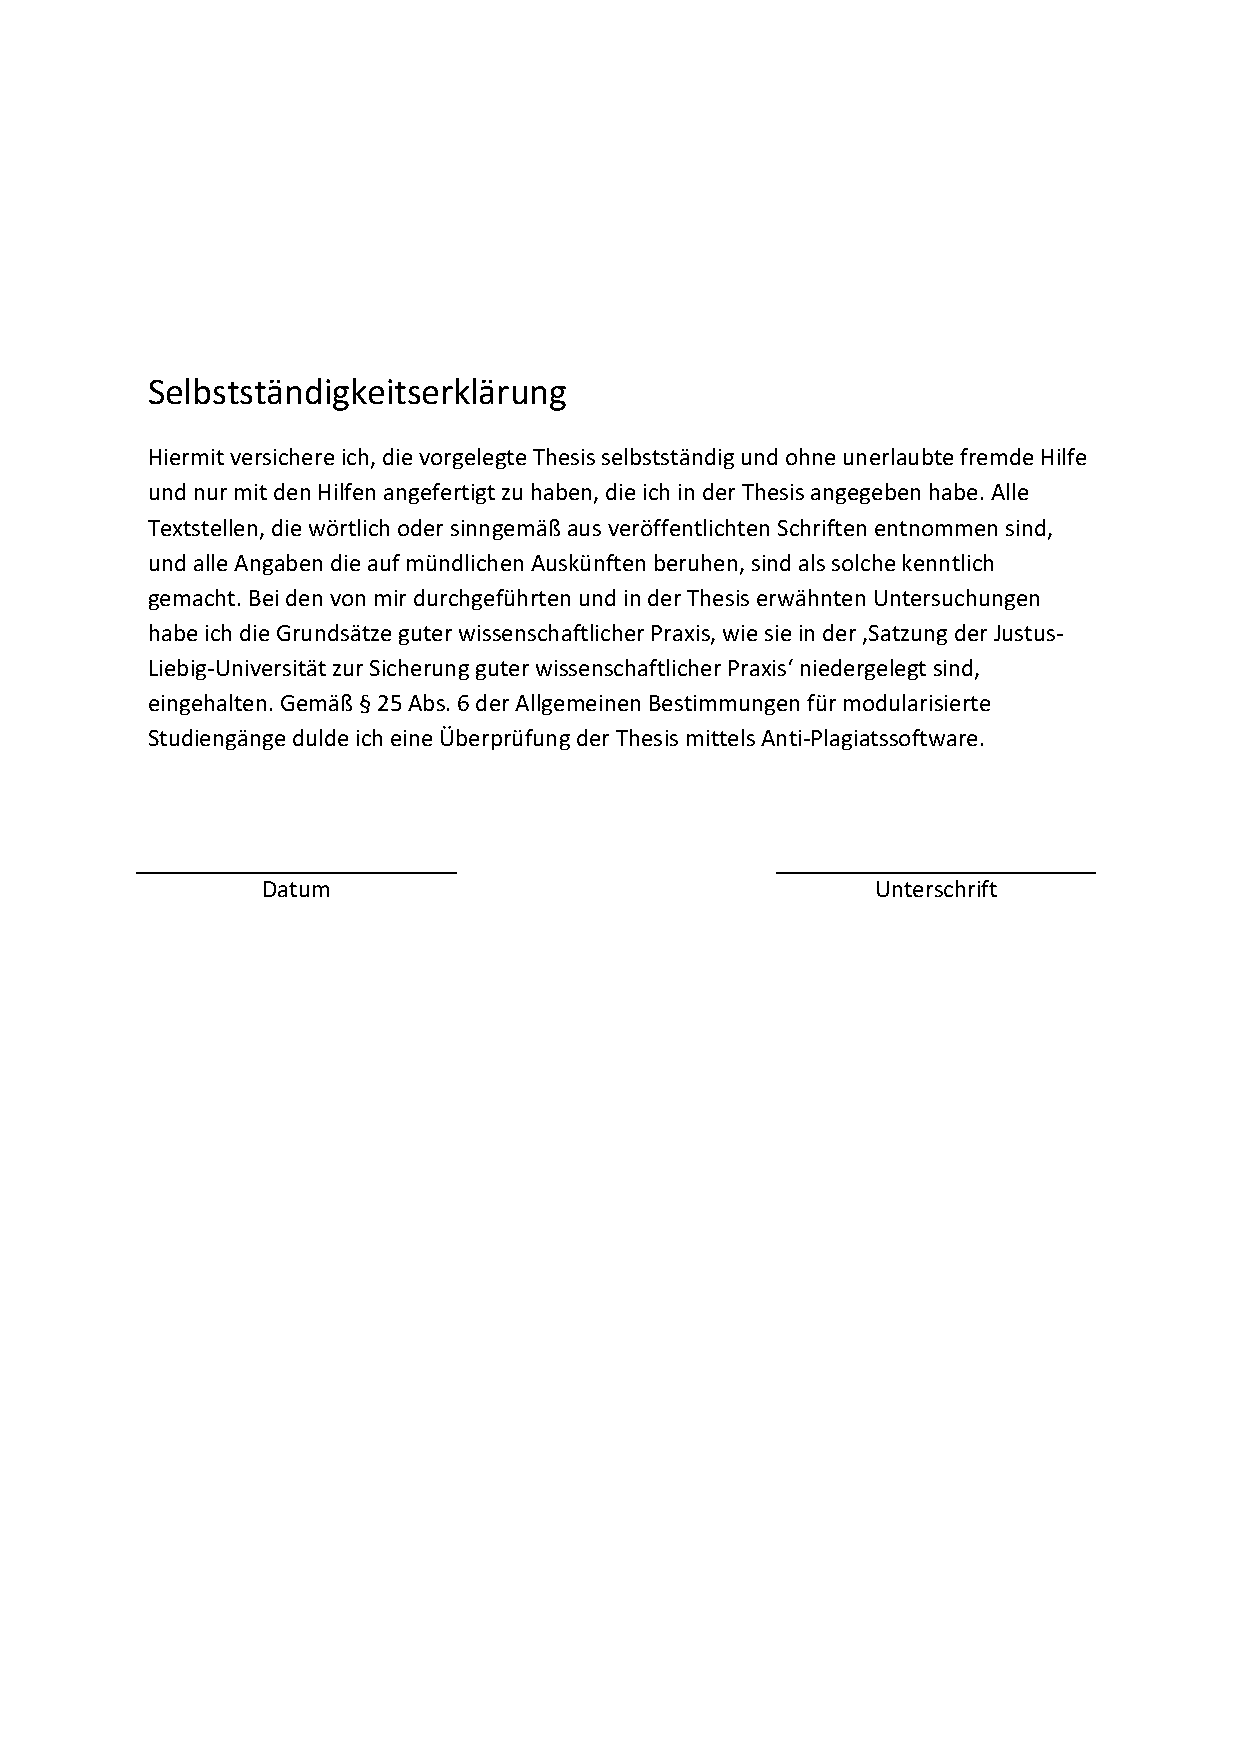
\includepdf[noautoscale=true, width=\paperwidth]{data/selbststaendigkeit.pdf}


\section{Introduction}
\subsection{Cosmic Radiation}
\acrfull{uhecr} is cosmic radiation with energy in the range of $10^{18}$\,eV to $10^{20}$\,eV.\footnote{The energy unit eV(Electron-Volt) describes the kinetic energy a unit charge holds after being accelerated through an electric field for 1V. It is equivalent to $1.602176634\cdot10^{-19}\,\text{J}$.}
Cosmic radiation has been discovered in 1912 by Viktor Hess by performing measurements with three electrometers in a balloon flight. He measured the energy flux in the atmosphere and showed that it increased with altitude. This is explained by secondary particles which are produced through the interaction of primary cosmic radiation with the atmosphere. The cosmic radiation is produced by many different sources, one of which is our sun. The sun however only produces cosmic radiation up to a few hundred MeV of energy through coronal mass ejections and other processes and so is not contributing to \acrshort{uhecr}. Higher energy sources include other stars, supernovae and also black holes. \\
\begin{figure}[ht!]
	\centering
	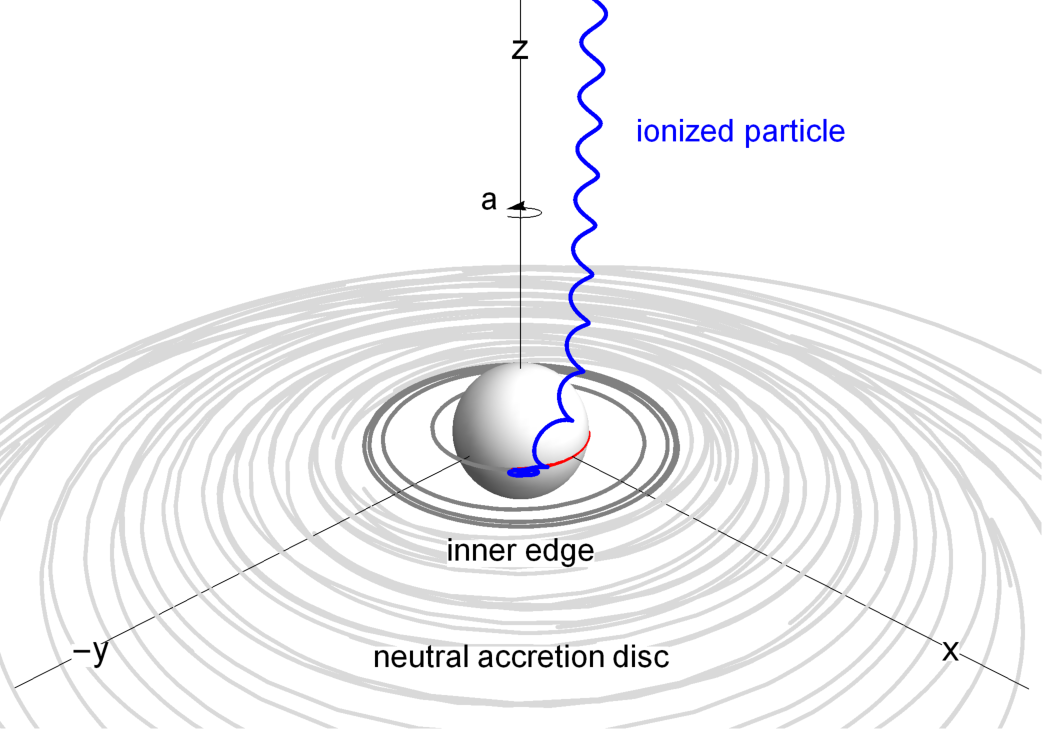
\includegraphics[width=0.5\linewidth]{data/uhecr-sm-bh}
	\caption{Trajectory of neutral particle around supermassive black hole \cite{Tursunov_2020}}
	\label{fig:uhecr-sm-bh}
\end{figure}\\
The production mechanisms for \acrshort{uhecr} are unknown and an area of active research, though some sources have been speculated. One such proposed mechanism is a spinning supermassive hole with a neutral particle in its accretion disk. The Orbit of this particle decays until it is close enough to the black hole so that the effective electric charge dominates and ionises the particle which causes a large acceleration\cite{Tursunov_2020}. The trajectory of the particle is shown in figure \ref{fig:uhecr-sm-bh}.\\
\begin{figure}[ht!]
	\centering
	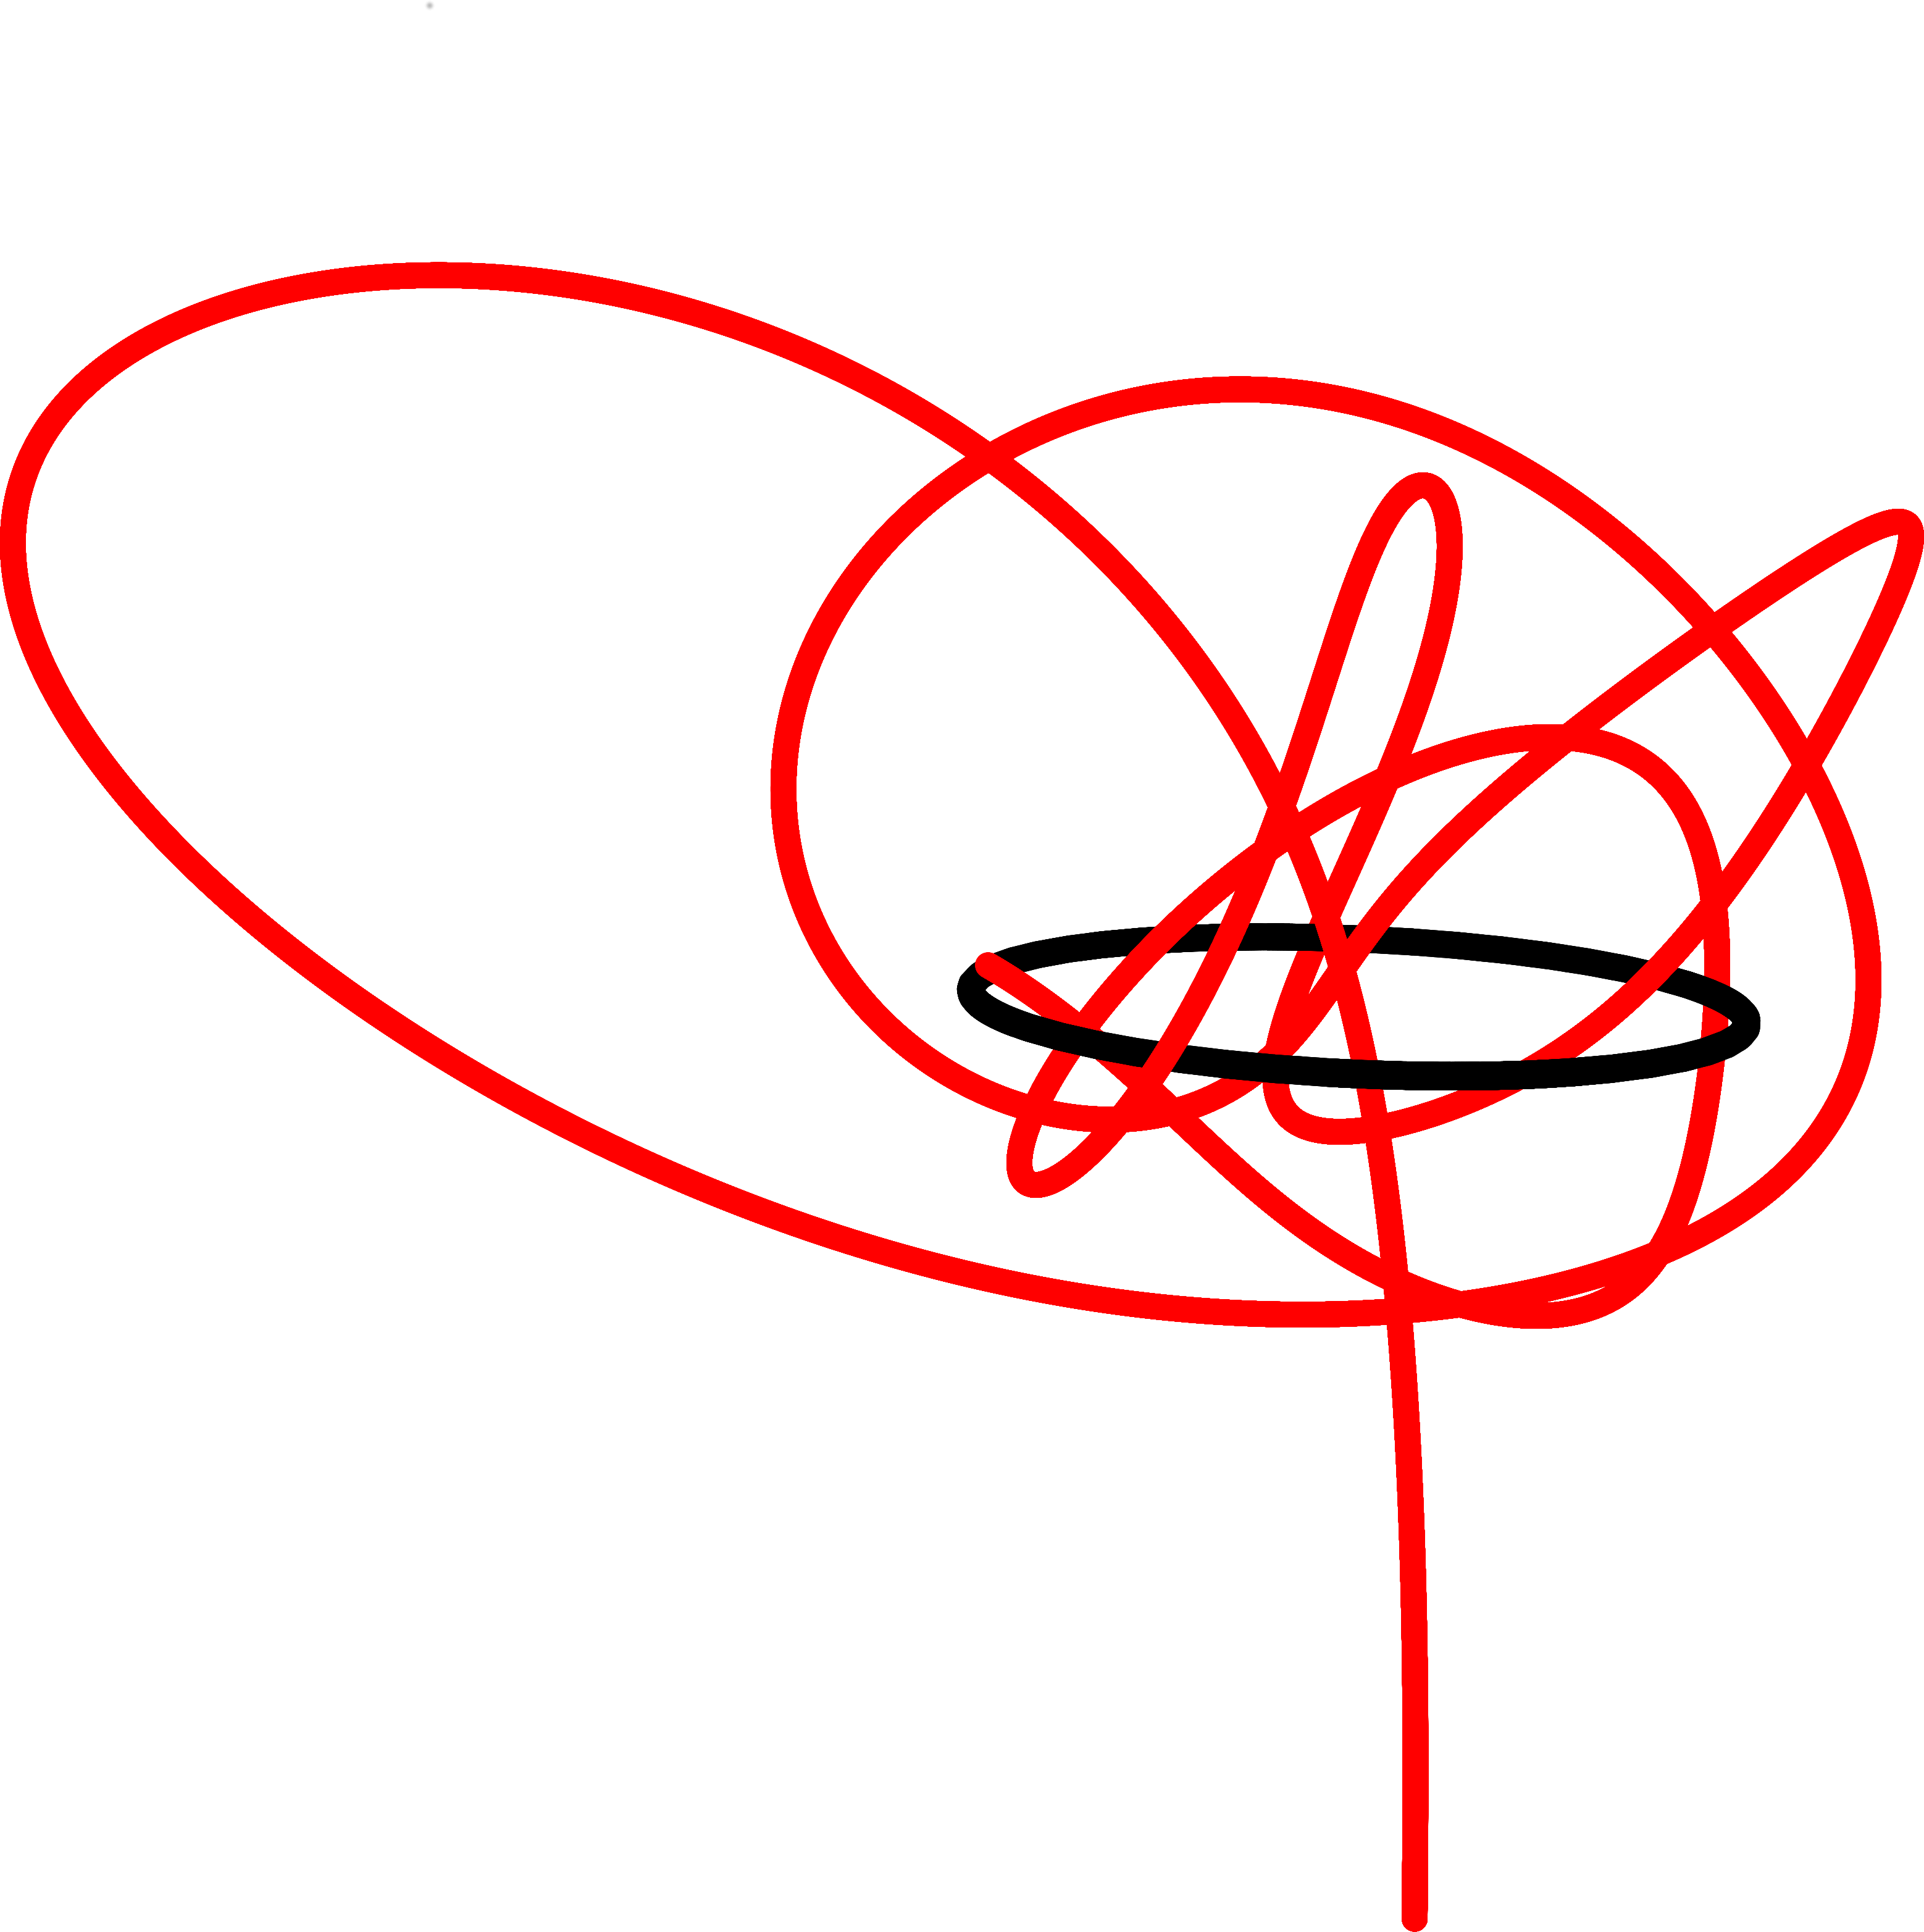
\includegraphics[width=0.4\linewidth]{data/trajectory-binary-bh}
	\caption{Possible trajectory of UHECR in Binary Black hole system \cite{Zhang2020}}
	\label{fig:trajectory-binary-bh}
\end{figure} \\
Already high energy particles can be accelerated to the ultra high energy regime. One possible acceleration mechanism relies on a pair of binary black holes which move at relativistic speeds. In such a scenario the particle can experience a series of gravitational slingshots \cite{Zhang2020} around the binary system and finally be accelerated so much it reaches the necessary energy region to be classified as an \acrshort{uhecr}. One possible trajectory of a particle that lead to an \acrshort{uhecr} which has been simulated is shown in figure \ref{fig:trajectory-binary-bh}. \\
\begin{figure}[ht!]
	\centering
	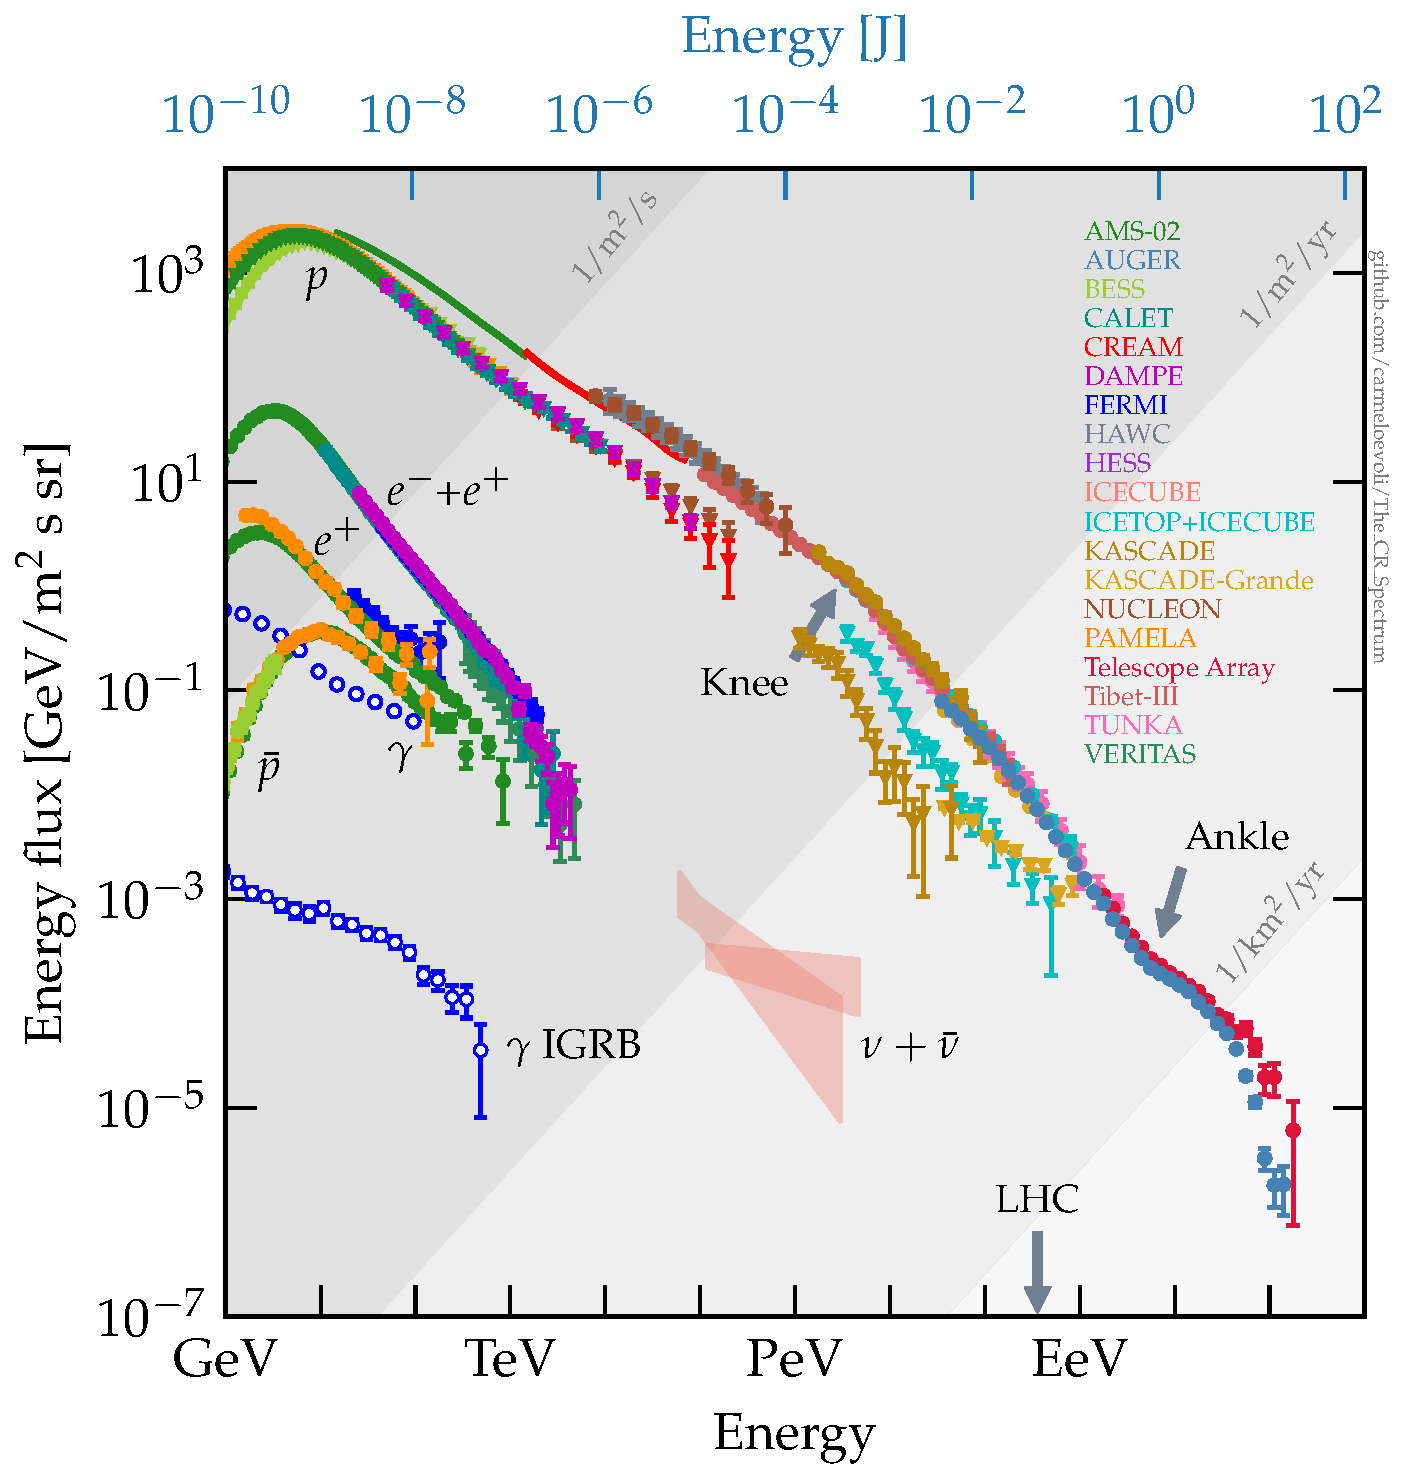
\includegraphics[width=0.75\linewidth]{data/cr_spectrum}
	\caption{Spectrum of cosmic radiation \cite{evoli_carmelo_2020_4396125}}
	\label{fig:cr_spectrum}
\end{figure} \\
The spectrum of this cosmic radiation is shown in figure \ref{fig:cr_spectrum}. There, measurements from different experiments are shown. The y axis shows the energy flux of cosmic rays in units of energy per second per square meter per solid angle $\frac{\text{GeV}}{\text{m}^2\cdot\text{s}\cdot\text{sr}}$. The x axis shows the primary energy of the cosmic rays, for comparison the upper axis shows the energy in units of Joule, the lower axis shows it in units of electron-Volt. Notable here is the much higher number of protons as compared to all other particles by two orders of magnitude. This allows one to make the reasonable assumption that most cosmic rays are protons. Prominent features of the proton spectrum are two anomalies labeled as Knee and Ankle. \\
One interesting observation is that the proton spectrum does not have a solid cutoff at $5\cdot10^{19}$\,eV of energy, rather it extends beyond it. This value is significant because it is calculated to be the \acrfull{gzkl}\cite{2021APh...12602526B}. This limit stems from high energy protons interacting with the microwave background radiation and being lifted into an excited state.
\begin{equation}\label{eq:gzkl}
	\begin{aligned}
		\gamma + p &\rightarrow \Delta^+ &\rightarrow p + \pi^0 \\
		\gamma + p &\rightarrow \Delta^+ &\rightarrow n + \pi^+
	\end{aligned}
\end{equation}
Equation \ref{eq:gzkl} descibes the possible interaction between the microwave background photons and protons. In both cases, the proton gets excited to a $\Delta^+$ resonance state, which can decay to a hadron and a pi meson. One possible decay product is a proton and a $\pi^0$, the other one a neutron and a $\pi^+$. In this process, the proton loses roughly $20\,\%$ of its energy, since the energy prior to the interaction gets transferred to both resulting particles according to their relative masses. Should the proton then remain above the limit, the same interaction can take place again. It is unlikely that any proton at these energies can travel more than $100\,\cdot10^6\,\text{ly}$ without undergoing this interaction. Since most particles above the ankle in the proton specturm shown in figure \ref{fig:cr_spectrum} are of extragalactic origin, this means that virtually all protons with these high energies must have undergone this interaction, dropping them below the \acrshort{gzkl}.
The violation of this limit could be explained with a proposition by the Pierre Auger Observatory that most \acrshort{uhecr} are in fact heavier nuclei than single protons \cite{thepierreaugercollaboration2017inferences}.

\subsection{Cosmic Air Showers}\label{subsec:airshowers}
When a cosmic ray hits the atmosphere, it interacts with the nucleons of the different molecules in air. Due to the relative abundance, it is most likely that the first interaction takes place between the primary particle and a Neutrogen nucleus. This causes interactions described by Quantum Chromo dynamics which is beyond the scope of this thesis. This interaction leaves nucelar fragments and $\pi$ mesons behind which can then interact with other air molecules again or - in the case of pions - decay. This creates a cascade of particles which continue along the trajectory towards the surface of earth. A picture of an air shower produced by a primary proton is shown in figure \ref{fig:proton-shower}. This image is produced at the KIT with the simulation toolkit CORSIKA.
\begin{figure}[ht!]
	\centering
	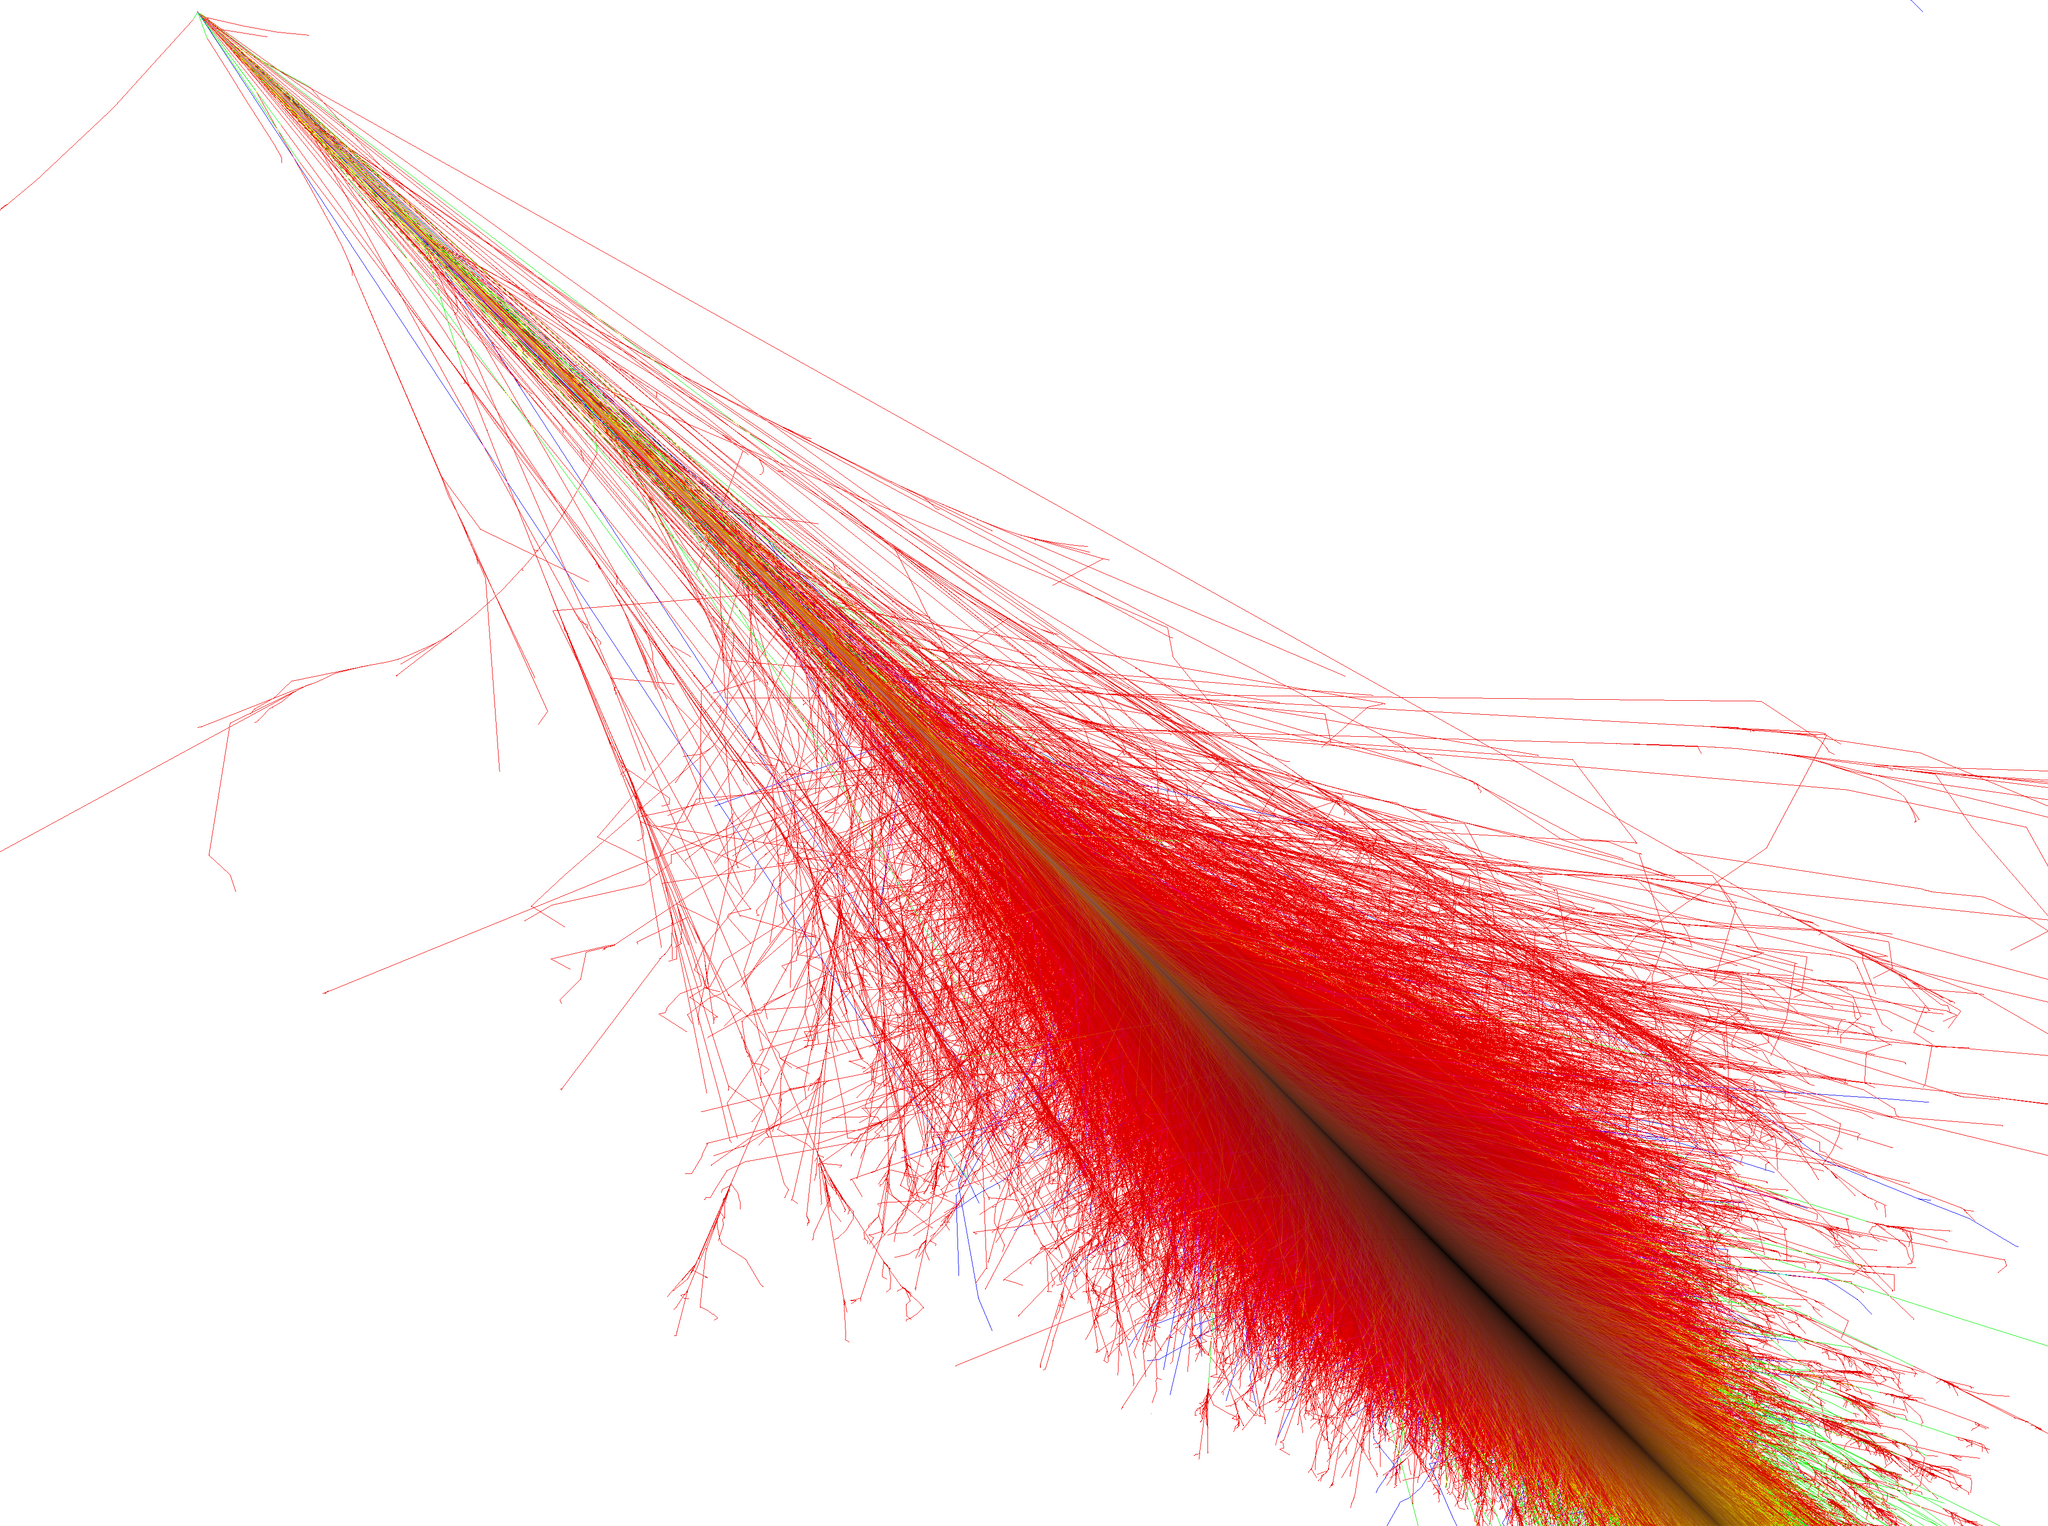
\includegraphics[width=0.8\linewidth]{data/shower-45}
	\caption{Proton Air Shower \cite{corsika-images}}
	\label{fig:proton-shower}
\end{figure} \\

The secondary particles can be divided into three different components, they are shown in figure \ref{fig:shower-components}.
As seen in this figure, neutral Pions $\pi^0$ can decay to two photons $\gamma$ or an electron positron pair and a photon. The decay cross section for the two gamma production is much higher than that of the $e^\pm + \gamma$ production though, resulting in probabilities of roughly $99$ and $1\,\%$. 
\begin{equation}
	\begin{aligned}
		\pi^0 &\rightarrow 2\gamma \\
		\pi^0 &\rightarrow e^+ + e^- + \gamma \\
	\end{aligned}
\end{equation}
The produced photons can then undergo pair production through which a lepton - anti lepton pair is produced. For this to occur, the photon needs to have an energy higher than twice the rest mass of the lepton. In the case of an electron positron pair, the rest energy is $511\,\text{keV}$ resulting in a minimum photon energy of $1022\,\text{keV}$. Any energy above this limit gets distributed evenly across both resulting particles as kinetic energy. In the \acrfull{com} system due to conservation of impulse, the pair travels in opposite directions to each other in a 90 degree angle to the original photon. In the laboratory system however, the resulting particles continue along the original trajectory.
\todo{sources for decay probabilities}
Should the photon not have enough energy to produce a pair, it can be absorbed in an atom by raising the energy level of an electron in the shell or loose energy through Compton scattering.\\
In the case of a charged pion $\pi^\pm$, The most likely decay with a probability of $99.9\,\%$ is to a muon $\mu^\pm$ and a muon-neutrino $\nu_\mu$. The interaction is shown in equation \ref{eq:piondecay}.
\begin{equation}\label{eq:piondecay}
	\begin{aligned}
		\pi^+ &\rightarrow \mu^+ + \nu_\mu \\
		\pi^- &\rightarrow \mu^- + \bar{\nu}_\mu
	\end{aligned}
\end{equation}
\begin{figure}[ht!]
	\centering
	\begin{tikzpicture}
		\draw[->] (0,0.5) node[above] {primary particle} -- ++(0,-1.5) coordinate(primary);
		\draw[->] (primary) -- ++(-175:1.5) node[above] {$\pi^0$} -- ++(-175:2) coordinate (pi0);
		\draw[->] (primary) -- ++(-105:1) node[left] {$\pi^\pm$} -- ++(-105:1.5) coordinate (pipm);
		\draw[->] (primary) -- ++(-35:1) -- ++ (-35:2) coordinate (zn);
		
		\draw[->] (pi0) -- ++(-160:1) coordinate(gamma) node[above right] {$\gamma$};
		\draw[->] (pi0) -- ++(-130:1) node[below right] {$\gamma$};
		\draw[->] (gamma) -- ++(-165:1) node[above] {$e^\pm$};
		\draw[->] (gamma) -- ++(-155:1) node[below] {$e^\mp$};
		
		\draw[->] (pipm) -- ++(-110:1) node[left] {$\mu^\pm$};
		
		\draw[->] (zn) -- ++(-10:1) node[above] {p};
		\draw[->] (zn) -- ++(-30:1) node[below] {n};
		
		\draw[thin, dashed] (-2,0) -- ++(0,-5) ++ (-0.5,0) node[left] {Electromagnetic};
		\draw[thin, dashed] (2,0) -- ++(0,-5) ++(-1,0) node[left] {Muonic} ++(1.5,0) node[right] {Hadronic};
	\end{tikzpicture}
	\caption{Components of a cosmic air shower}
	\label{fig:shower-components}
\end{figure}
\todo{further specify EAS}
The figure does not show all interactions, nor does it show the Neutrinos produced through the different interactions.
The shower impact is dependent on the type of primary particle and its energy. In the case of \acrshort{uhecr}, the showers are classified as \acrfull{eas}.

Additionally to cosmic air showers, the primary particles produce Cherenkov radiation. This is light in the UV spectrum which results from the particles traveling faster than the local speed of light. This is an effect comparable to the sonic cone for objects traveling faster than the speed of sound in a medium like air.
\begin{figure}[ht!]
	\centering
	\begin{tikzpicture}
		\draw[->] (0,0) -- ++(1,0) node[above left] {$v$};
		\draw (0,0) -- ++(7,0) coordinate (tip);
		
		\draw (tip) -- ++(135:4) -- ++(-135:2) coordinate(top) -- ++(-135:2);
		\draw[dashed, ->] (tip) ++(135:1.0) -- ++(45:1);
		\draw[dashed, ->] (tip) ++(135:1.5) -- ++(45:1);
		\draw[dashed, ->] (tip) ++(135:2.0) -- ++(45:1);
		\draw[dashed, ->] (tip) ++(135:2.5) -- ++(45:1);
		\draw[dashed, ->] (tip) ++(135:3.0) -- ++(45:1);
		\draw[dashed, ->] (tip) ++(135:3.5) -- ++(45:1);
		
		\draw (tip) -- ++(-135:4) -- ++(135:4);
		\draw[dashed, ->] (tip) ++(-135:1.0) -- ++(-45:1);
		\draw[dashed, ->] (tip) ++(-135:1.5) -- ++(-45:1);
		\draw[dashed, ->] (tip) ++(-135:2.0) -- ++(-45:1);
		\draw[dashed, ->] (tip) ++(-135:2.5) -- ++(-45:1);
		\draw[dashed, ->] (tip) ++(-135:3.0) -- ++(-45:1);
		\draw[dashed, ->] (tip) ++(-135:3.5) -- ++(-45:1);
		
		\draw[<->] (top) arc(45:22.5:2) coordinate(theta) arc(22.5:0:2);
		\node[below left] at (theta) {$\theta$};
	\end{tikzpicture}
	\caption{Geometry of cherenkov radiation. Dashed are the UV photons, the angle $\theta$ is dependent on the incident particle velocity $v$ and the refractive index $n$ of the medium.}
	\label{fig:cherenkov}
\end{figure}
\clearpage
\subsection{Detection methods}

The detection of \acrshort{uhecr} can be done through three main methods.\\
Two depend on the cosmic air showers described in the section \ref{subsec:airshowers}, namely the muonic and the electromagnetic component. The other method depends on the Cherenkov radiation.
In the case of Cherenkov radiation, UV telescopes can be used to detect the UV light directly. By observing the same source through multiple locations, the origin can be reconstructed. 
A popular example of a particle being detected through these means is the so called Oh-My-God particle, likely a proton or heavier nucleus with an energy of  $3.2\pm0.9\cdot10^{20}\,\text{eV}$ of energy. This particular particle is interesting since it was the first particle to exceed the \acrshort{gzkl}. It has been detected by the HiRes detector in Utah.

A method using the electromagnetic component of a cosmic air shower exploits the fact that the frequencies lie in the radio range\cite{NELLES201513} and can be detected through normal radio Antennae\cite{SCHRODER20171}. Due to the polarisation of the radio signal, often multiple antennae with different polarisation characteristics are used.


\begin{figure}[ht!]
	\centering
	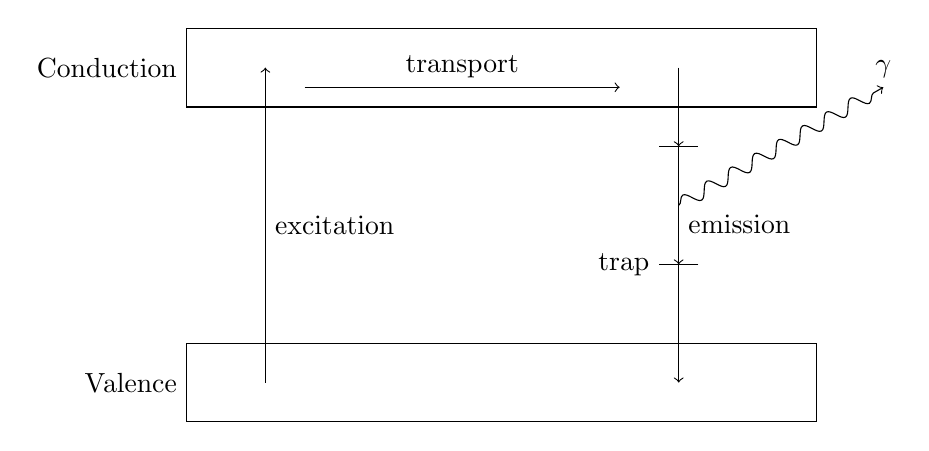
\begin{tikzpicture}[->]
		\draw (0,0) rectangle++(8,1);
		\draw (0,-3) rectangle++(8,-1);
		
		\draw (1,-3.5) -- ++(0,2) node[right] {excitation} -- ++(0,2);
		
		\draw (1.5,0.25) -- ++(2,0) node [above] {transport} -- ++(2,0);
		
		\draw[-] (6,-0.5) -- ++(0.5,0);
		\draw[-] (6.5,-2) -- ++(-0.5,0) node [left] {trap};
		
		\draw (6.25,0.5) -- ++(0,-1);
		\draw (6.25,-0.5) -- ++(0,-0.75) coordinate(emission) -- ++(0,-0.75);
		\draw (6.25,-2) -- ++(0,-1.5);
		
		\draw[decorate, decoration=snake] (emission) -- ++(30:3) node [above] {$\gamma$};
		\node[below right] at (emission) {emission};
		
		
		\node[left] at (0,0.5) {Conduction};
		\node[left] at (0,-3.5) {Valence};
	\end{tikzpicture}
	\caption{Mechanism for crystal scintillators}
	\label{fig:scintillator}
\end{figure}
Another method is to detect the muonic component, this can be done through Scintillator detectors. Due to the muon being a charged particle, it interacts with matter and deposits energy. Certain materials can give off this energy via photons, a process which is known as scintillation. Figure \ref{fig:scintillator} shows the mechanism through which scintillation occurs. First, an electron is excited from the valence band into the conduction band through energy deposit from an incident particle. This electron then is transported through the conduction band where it can drop back down to the valence band. Though if it dropped back directly, a photon would be emitted which could immediatly excit another electron in the valence band. What makes scintillators special is the existance of traps which reduce the energy of the emitted photons. Those photons then do not have enough energy to excite eletrons in the material so they can pass through it. With the use of a photmultiplier, the emitted photons can then be detected. One type of Photomultiplier is the \acrfull{sipm}, which is an array of single-photon avalanche diode which are photodiodes operating above the reverse-bias breakover voltage resulting in an avalanche upon interaction with even a single photon. The multiplicity of avalanches then is related to the number of photons interacting with the photmultiplier.
\section{Detector Network}
Since one detector alone only provides the timestamp of one particle hit, it does not provide useful information on its own when the goal is to measure cosmic shower events. That is why for real measurements a network of detectors has to be used. The network on which this thesis is based consists of low-cost plastic scintillator detector units utilising a Raspberry Pi minicomputer add-on board as readout electronics. Those detectors are specifically intended as a citizen science project. This has the benefit of being able to distribute detectors over a large area with minimal resource use.


Each detector in the network consists of a scintillator with \acrfull{sipm} assembly, an interface board with \acrfull{adc} and a Raspberry Pi minicomputer. The interface board receives signals from the \acrshort{sipm} and records the current timestamp. This timestamp is then processed by a software running on the Raspberry Pi minicomputer which sends it to a server. Each timestamped event is thus written to a central database where it can be further analysed at a later time. Due to the number of detectors and their respective rate of few Hz each, a large number of events is written to the database. In set intervals, this Data is analysed through post-processing methods. This however puts a large strain on the server infrastructure due to the amount of data being read and written back to the database. A better approach is to perform a pre-processing step through a filter before storing each the data point in the database.
\begin{figure}[ht!]
	\centering
	\begin{tikzpicture}[>=latex, ->]
		\node (scintillator) [draw, process, minimum height=1cm] {Scintillator};
		\node (sipm) [right=of scintillator, draw, process, minimum height=1cm] {SiPM};
		\node (cdu) [right=of sipm, draw, process, minimum height=1cm] {CDU};
		\node (rapi) [right=of cdu, draw, process, minimum height=1cm] {Raspberry Pi};
		\node (server) [below=of rapi, draw, process, minimum height=1cm] {Server};
		\node (dnp) [left=of server, draw, process, minimum height=1cm] {DNP};
		\node (db) [left=of dnp, draw, process, minimum height=1cm] {Database};
		
		\draw (scintillator) -- (sipm);
		\draw (sipm) -- (cdu);
		\draw (cdu) -- (rapi);
		\draw (rapi) -- (server);
		\draw (server) -- (dnp);
		\draw (dnp) -- (db);
	\end{tikzpicture}
	\caption{Path of one event through the detector network}
	\label{fig:event-path}
\end{figure}
The path of an event through the detector network is shown in figure \ref{fig:event-path}. There, CDU stands for Cosmic Detector Unit, which is the hardware add-on board on top of the Raspberry Pi. DNP stands for Detector Network Processor, the software running on the server which analyses each event.

\subsection{Data}
The shower front shape of a cosmic shower can initially be assumed to be a thick spherical cap with a thickness of $1\,\text{to}\,2\,\text{m}$\cite{grapes-3-2019}. This shape however fluctuates between shower events and measurements range from spherical cap shapes\cite{chitnis-2002} to conical shapes\cite{grapes-3-2019}. The thickness and deviation from the shape of a spherical cap introduce uncertainties in the calculations presented in this thesis in section \ref{sec:reconstruction}.
\begin{figure}[ht!]
	\centering
	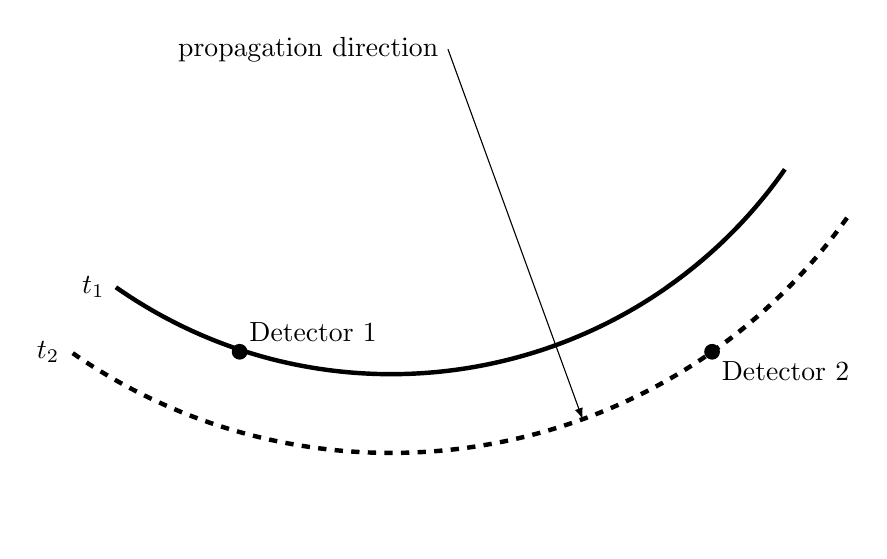
\begin{tikzpicture}
		\fill (0,0) coordinate(det1) circle(0.1) node[above right] {Detector 1};
		\fill (6,0) coordinate(det2) circle(0.1) node[below right] {Detector 2};
		\draw[ultra thick] (det2) ++ (125:1) arc(-55:-35:6.1) arc(-35:-125:6.1) node[left] {$t_1$};
		\draw[ultra thick, dashed] (det2) arc(-55:-35:7.1) arc(-35:-125:7.1) node[left] {$t_2$};
		\path (det2) arc(-55:-70:7.1) coordinate(source);
		\draw[<-, >=latex] (source) -- ++ (110:5) node[left] {propagation direction};
	\end{tikzpicture}
	\caption{Propagation of the shower front}
	\label{fig:data-shape}
\end{figure}
Figure \ref{fig:data-shape} shows the propagation of the shower front in relation to two detectors. Assuming both detectors have a detection efficiency of $100\,\%$, both will show an event at their respective timestamps $t_1$ and $t_2$. The time difference between both measured timestamps can help to reconstruct the direction of propagation, a method how to do this is shown later in this thesis.

Comparing the timestamps of single detector hits can be used to correlate single data points and combine them to coincidences.
\begin{figure}[ht!]
	\centering
	\begin{tikzpicture}
		\begin{axis}[area style, xlabel={$\Delta{t}\,[\text{ns}]$},ylabel={$n$}, xmin=-150,xmax=150]% coordinates
			\addplot+[ybar interval,mark=no] table {data/hgz0_hgzHeuchelheim2.hist};
		\end{axis}
	\end{tikzpicture} \\
	\begin{tikzpicture}
		\draw[ultra thick] (1,0) -- ++(-1,0) node [left] {Detector 1};
		\draw[ultra thick] (4,4) -- ++(1,0) node [right] {Detector 2};
		
		\draw (1,0) -- ++ (4,0);
		\draw[<->] (4.9,0) -- ++ (0,4);
		\draw (0.5,0) -- ++(0,5);
		\draw (4.5,4) -- ++(0,1);
		\draw[<->] (0.5,4.9) -- ++ (4,0);
	\end{tikzpicture}
	\caption{Coincidence time histogram for two detector pairs with geometric}
	\label{fig:histogram-data}
\end{figure}
When recording all coincidence times of one detector pair the different times can be plotted in a histogram. Figure \ref{fig:histogram-data} shows the geometrical arrangement and the histogram of coincidence data. Due to the close distance between both detectors, a large peak with Gaussian distribution can be seen which is significantly higher than the background which comprises of random coincidences due to noise in the \acrshort{sipm}. In the figure an offset can be observed which is due to hardware limitations in the detector setup.
\todo{complete figure \ref{fig:histogram-data}}
\section{Real-time analysis}
In order to detect coincidences from all incoming single data points, each data point has to be compared with all others in order to find all possible combinations. In order to do this, a useful criterium for a coincidence has to be found. A simple approach is to select a fixed maximum time difference which two events can have in order to be counted towards a coincidence. This however is inefficient and leads to large numbers of false positives, since a fixed interval can not perform well for detector combinations with large and short distances at the same time. Due to this a variable distance based criterium is used. For this purpose, the geodetic coordinates of both detector stations are taken and the straight line distance is calculated through \acrfull{enu} coordinates with the WGS84 model. The \acrshort{enu} coordinate system is a right handed local tangent plane carthesian coordinate system $\left(\hat{e}_{East},\hat{e}_{North},\hat{e}_{Up}\right)$ which is used to set different coordinates in relation to each other. The WGS84 model describes the shape of earth as an ellipsoid and provides reference measurements for this shape.

With this distance, the time of flight for the speed of light is calculated in order to receive the maximum physically viable time difference for one detector pair. This value however has large uncertainties especially for detector pairs which are close together.

Since there is a constant timing offset of a few nanoseconds for each detector pair which arises through the specific hardware setup, a minimum coincidence window must be defined in order to capture coincidences even for pairs with a large offset. A practical value of $150\,\text{ns}$ has been chosen.

It is also necessary to define an upper window, since the range of muons in air is limited and detector pairs with extremely large distances would create an abnormal and unphysical number of coincidences if left unconstrained. In order to find a useful upper limit for the coincidence window, the maximum possible flight distance for atmospheric muons has to be detemined. For that, the expected maximum range of muons in air is calculated. In order to do that, first a maximum expected energy is determined through the muon energy spectrum at sea level. Figure \ref{fig:muon-energy-spectrum} shows the muon energy spectrum at sea level for two different inclinations. A cutoff value of $10\,\text{TeV}$ is selected to calculate the maximum expected distance in air. Assuming the \acrfull{csda} range for a $10\,\text{TeV}$ muon taken from \cite{muon-range} of $7.634\cdot10^5\,\frac{\text{g}}{\text{cm}^2}$ and assuming standard condition air density of $1.225\,\frac{\text{kg}}{\text{m}^3}$, the maximum expected range of muons at sea level is $62.3\,\text{km}$. That equates to a time of flight of $207.87\,\mu\text{s}$ and thus a coincidence window of larger than that is not useful.
\begin{figure}
	\centering
	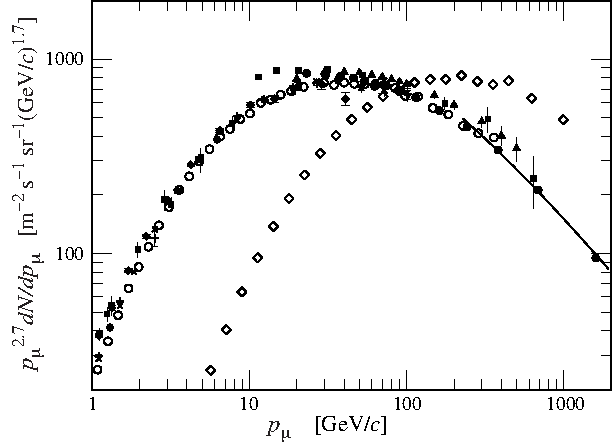
\includegraphics[width=0.7\linewidth]{data/cr_fig5_SeaLevelMuSpectra_09}
	\caption[Muon energy spectrum from vertical and inclined muons at sea level\cite{10.1093/ptep/ptaa104}]{Muon energy spectrum from vertical and inclined \tikz \draw[rotate=45] (0,0) rectangle(0.125,0.125); muons at sea level \cite[512]{10.1093/ptep/ptaa104}}
	\label{fig:muon-energy-spectrum}
\end{figure}
\subsection{Coincidence and plausability determination}
In order to determine coincidences, each event needs to be checked against all other events which are currently in the event buffer. To determine whether two events contain a coincidence, it is beneficial to calculate a score for each pair as follows:
\begin{equation}\label{eq:coinc_score}
	c = 1 - \frac{|t_1 - t_2|}{t_{tof}}
\end{equation}
In equation \ref{eq:coinc_score} $t_1$ and $t_2$ denote the timestamps of both events and $t_{tof}$ the time of flight between both stations. This results in a number $c\leq1$ where a value $\leq0$ describes an unphysical coincidence. In the case that multiple stations need to be compared, a complete graph needs to be calculated with edge weights equalling the score of the pair connected by this edge. An example of this construction is shown in figure \ref{fig:conflicts}.
\begin{figure}[ht!]
	\centering
	\begin{tikzpicture}
		\draw[ultra thick, -> , >=latex] (0,0) -- ++(10,0) node[below] {$t$};
		\draw[dashed] (1,0.5) -- ++(0,-1) node[below] {$t_1$};
		\draw[dashed] (3,0.5) -- ++(0,-1) node[below] {$t_2$};
		\draw[dashed] (5,0.5) -- ++(0,-1) node[below] {$t_3$};
		\draw[dashed] (8,0.5) -- ++(0,-1) node[below] {$t_4$};
		
		\node (s1) [networknode] at (0, -2) {$s_1$};
		\node (s1r) [right=of s1] {};
		\node (s1b) [below=of s1] {};
		\node (s2) [networknode, below=of s1b] {$s_2$};
		\node (s3) [networknode, below right=of s1r] {$s_3$};
		\node (s3r) [below right=of s3] {};
		\node (s4) [networknode, below=of s3r] {$s_4$};
		
		\path[draw]
			(s1) edge node[left] {$c_{12}$} (s2)
			(s1) edge node[above] {$c_{13}$} (s3)
			(s2) edge node[left] {$c_{23}$} (s3)
			(s3) edge node[above right] {$c_{34}$} (s4)
			;
		\path[draw, dashed]
			(s1) edge node[below] {$c_{14}$} (s4)
			(s2) edge node[below] {$c_{13}$} (s4)
			;
		
	\end{tikzpicture}
	\caption{Visualisation of four single events with possible coincidences}
	\label{fig:conflicts}
\end{figure}
There, \tikz \draw (0,0) -- (0.5,0); marks a physical time difference and \tikz \draw[dashed] (0,0) -- (0.5,0); marks an unphysical time difference. This leads to a conflict, since all stations $s_{1,2,3,4}$ have at least one physical coincidence time to at least one other station, but the data for $s_4$ only fits together with the data of $s_3$. This means that the whole coincidence is not physically viable, though an unknown number of partial coincidences can be.

In order to quantify this problem as one number, the unweighted plausibility score is introduced. Consider the graph with vertices $V = (s_1; s_2; s_3; s_4)$ from figure \ref{fig:conflicts} where the edges describe possible coincidences and the vertices detector stations. Only the set of edges $E = (c_{12}; c_{13}; c_{23}; c_{24})$ contains valid coincidences. The plausibility score of a full event with $n$ detector stations is then defined through
\begin{equation}
p = \frac{|E|}{\Delta_{n-1}}=\frac{2\cdot|E|}{n(n-1)}
\end{equation}
where $\Delta_n$ is the triangular number and $|E|$ the number of edges in the set $E$.

For a fully plausible coincidence event, this score is $1$, for the example in figure \ref{fig:conflicts} it is $p = \frac{4}{6}=\frac{2}{3}$.

In order to attempt to resolve this conflict additionally the weighted plausibility score $_wp$ is introduced:
\begin{equation}
	_wp = \frac{\sum^{n}_{i}\sum^{n}_{j} c_{ij}}{\Delta_{n-1}}
\end{equation}

The goal in resolving conflicting data is to maximise $_wp$ and reach $p=1$. Without access to more data is is impossible to definitively resolve this conflict, however an approximation can be performed.

This approximation can be done through selectively removing the vertex $s_i$ with lowest weighted rank
\begin{equation}
_wrank(s_i) = \sum_{j}^{n}c_{ij}
\end{equation}
in the graph and recalculating $_wp$, this is repeated until $p=1$ is reached. Should this prove to be impossible without removing too many edges for the purpose of preserving potentially useful data the process is cancelled and the whole event is accepted tentatively.

\section{Primary reconstruction}\label{sec:reconstruction}
\subsection{Possible primary incident angles}
Through the assumptions shown in figure \ref{fig:angle-assumptions}, the possible source directions of a primary particle can be reduced. There, the geometry of a coincidence with $n=2$ is shown. Since she shower front can be simplified as a spherical section and the propagation speed can be assumed to be near the speed of light, two spheres with a shared tangent can be constructed. One spherical surface is the shower front, the other is a sphere around the detector which had the later event timing. Its radius $\ell$ is equal to the propagation time of light for the coincidence time. Through geometrical analysis of this arrangement, the Radius and angle pair can be derived as a function of the angle $\alpha$. This creates a curve in the plane on which the primary interaction must have taken place. Due to the symmetry of this arrangement however, in 3-D space, this curve becomes a rotational surface. \\
In the case of a coincidence with $n>2$ multiple curves can be calculated relative to the same root detector. This allows for the intersection points of each rotational surface to be calculated, which results in a reduced possible origin area for the primary interaction. \\
Given that the shower front is not a complete spherical surface but only a spherical section, the possible origin directions can be reduced with this approach. In the case of higher coincidence numbers, the possible direction can be reduced further. Additionally to the possible directions, this approach also provides a lower limit for the shower radius and footprint radius, suggesting a minimum Particle energy.
\begin{figure}[ht!]
	\centering
	\begin{tikzpicture}
		\fill (0,0) coordinate(det1) circle(0.1);
		\fill (6,0) coordinate(det2) circle(0.1);
		\draw (det2) circle(1);
		\draw (det2) -- ++(125:0.7) node[right] {$\ell$} -- ++(125:6.4) coordinate(center);
		\draw[dashed] (det2) ++(125:1) ++ (215:2) -- ++(35:4) node[right] {tangent};
		\draw (det2) ++ (125:1) arc(-55:-35:6.1) arc(-35:-125:6.1) node[left] {shower front};
		\draw (center) -- (det1) -- (det2);
		\draw (det2) ++(125:1) -- (det1);
		\draw (det2) ++(125:1) -- ++(0,1) -- ++(0,-2);
		
		\draw (det1) -- ++(0,-0.9) coordinate(det1b) -- ++(0,-0.1);
		\draw (det2) -- ++(0,-0.9) coordinate(det2b) -- ++(0,-0.1);
		
		\draw[<->] (det2b) -- (det1b);
		\node[above] at ($(det1b)!0.5!(det2b)$) {$d$};
		\node[above left] at ($(det1)!0.5!(center)$) {$r$};
		
		\draw[<->] (center) ++(-55:2) arc(-55:-108:2) node[above right] {$\delta$};
		\draw[<->] (det2) ++(125:2) arc(125:90:1) node[above left] {$\alpha$};
		\draw[<->] (det2) ++(125:2) arc(125:189:1) node[above right] {$\gamma$};
		\draw[<->] (det1) ++(0:1) arc(0:72:1) node[above right] {$\phi$};
		\draw[<->] (det1) ++(0:3) arc(0:8.584336297778657:3) node[below right] {$\beta$};
		\draw[<->] (det1) ++(8.584336297778657:3) node[above] {$s$};
		
	\end{tikzpicture}
	\caption{Assumption for possible incidence angles}
	\label{fig:angle-assumptions}
\end{figure}
Calculating the angles $\beta$ and $\gamma$ and length $s$, we get the equations
\begin{equation*}
	\beta = \arctan\left(\frac{\ell\cdot\cos\alpha}{d - \ell\sin\alpha}\right),
\end{equation*}
\begin{equation*}
	\gamma = \frac{\pi}{2} - \alpha + \beta
\end{equation*}
and
\begin{equation*}
	s = \sqrt{\left(l\cdot\cos\hspace{-2pt}\left(\alpha\right)\right)^2 + \left(d - l\cdot\sin\left(\alpha\right)\right)^2} = \sqrt{l^2 + d^2 - 2dl\sin\left(\alpha\right)}.
\end{equation*}
With those, the polar coordinates $(\phi, r)$ can be calculated with equations \ref{eq:phi} and \ref{eq:r}.
\begin{equation}\label{eq:phi}
	\phi = \gamma + \beta = \frac{\pi}{2} - \alpha + 2\cdot\beta
\end{equation}
\begin{equation}\label{eq:r}
	r = \frac{s}{2\cdot\cos\left(\gamma\right)} = \frac{\sqrt{l^2 + d^2 - 2{\cdot}d{\cdot}l{\cdot}\sin\left(\alpha\right)}}{2\cdot\sin\left(\alpha - \beta\right)}
\end{equation}


Figure \ref{fig:reconstruction_example} shows an example for possible combinations of $r$ and $\phi$ as calculated above for a detector pair with distance of $3.4\,\text{km}$ and a coincidence time of $7.37\,\mu\text{s}$. Following the curve, the free parameter $\alpha$ is varied. The minimum possible distance is reached when $\alpha=\frac{\pi}{2}$, since then the center of the constructed circle in figure \ref{fig:angle-assumptions} lies directly on the line between both detectors. As $\alpha$ approaches $0$, the possible radius tends to infinity and $\phi$ tends to a stationary value $\phi_\infty$.
\begin{figure}[ht!]
	\centering
	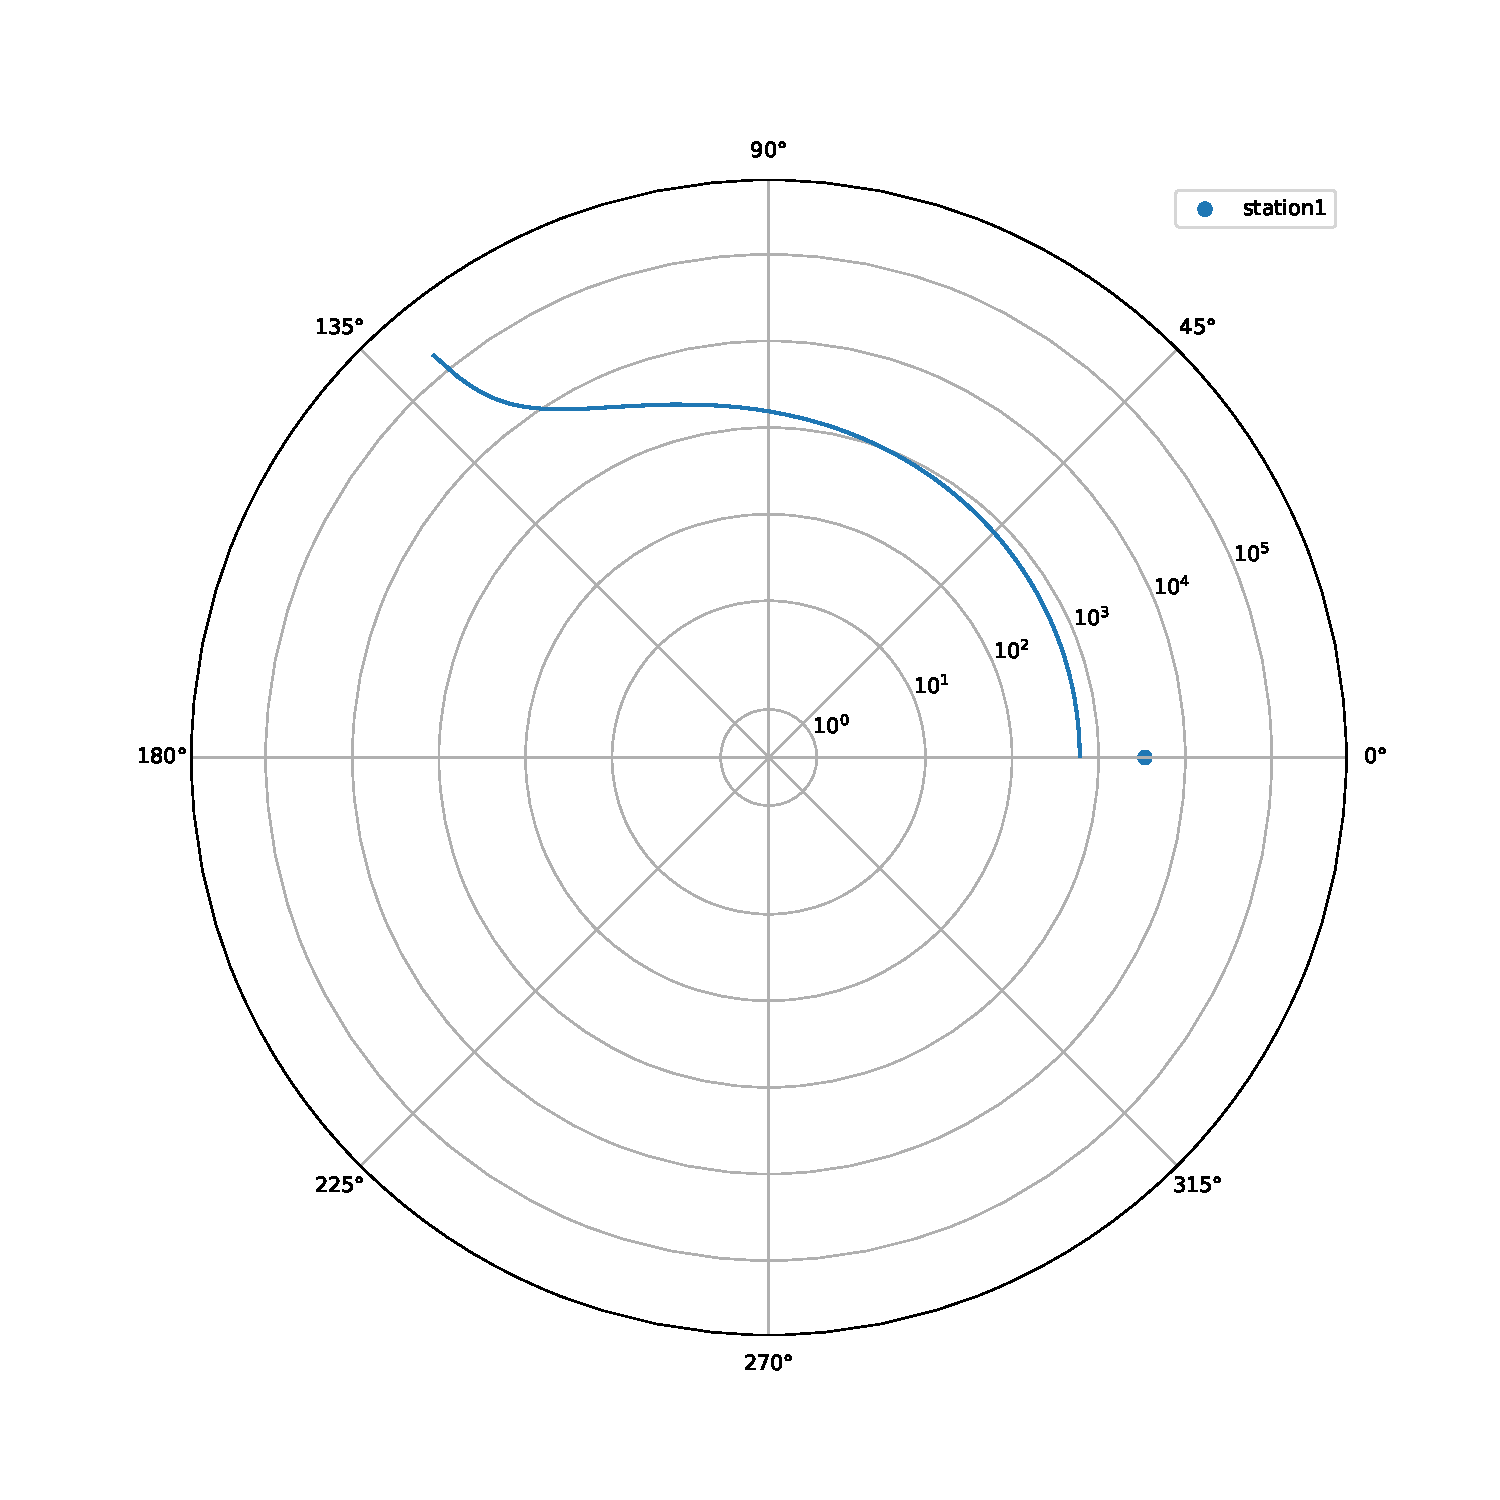
\includegraphics[width=0.4\linewidth]{data/example_plot_vertical}
	\caption{Plot of an example to reconstruct the possible direction of incident primary particle}
	\label{fig:reconstruction_example}
\end{figure}
\begin{equation*}
	\begin{aligned}
		\lim_{\alpha\rightarrow0}r\left(\alpha\right) &= \infty\\
		\lim_{\alpha\rightarrow0}\phi\left(\alpha\right) &= \phi_\infty
	\end{aligned}
\end{equation*}
Noteworthy is that the possible values for $\alpha$ are constrained by a maximum value for $\delta$ due to a maximum shower footprint on earth. Adjusting for that, a lower limit for the radius r can be calculated iteratively through equation \ref{eq:delta_alpha}.
\begin{equation}\label{eq:delta_alpha}
	\delta = \pi - 2\cdot\gamma = 2\cdot\alpha - 2\cdot\arctan\left(\frac{\ell\cdot\cos\alpha}{d - \ell\sin\alpha}\right)
\end{equation}
\begin{figure}[ht!]
	\centering
	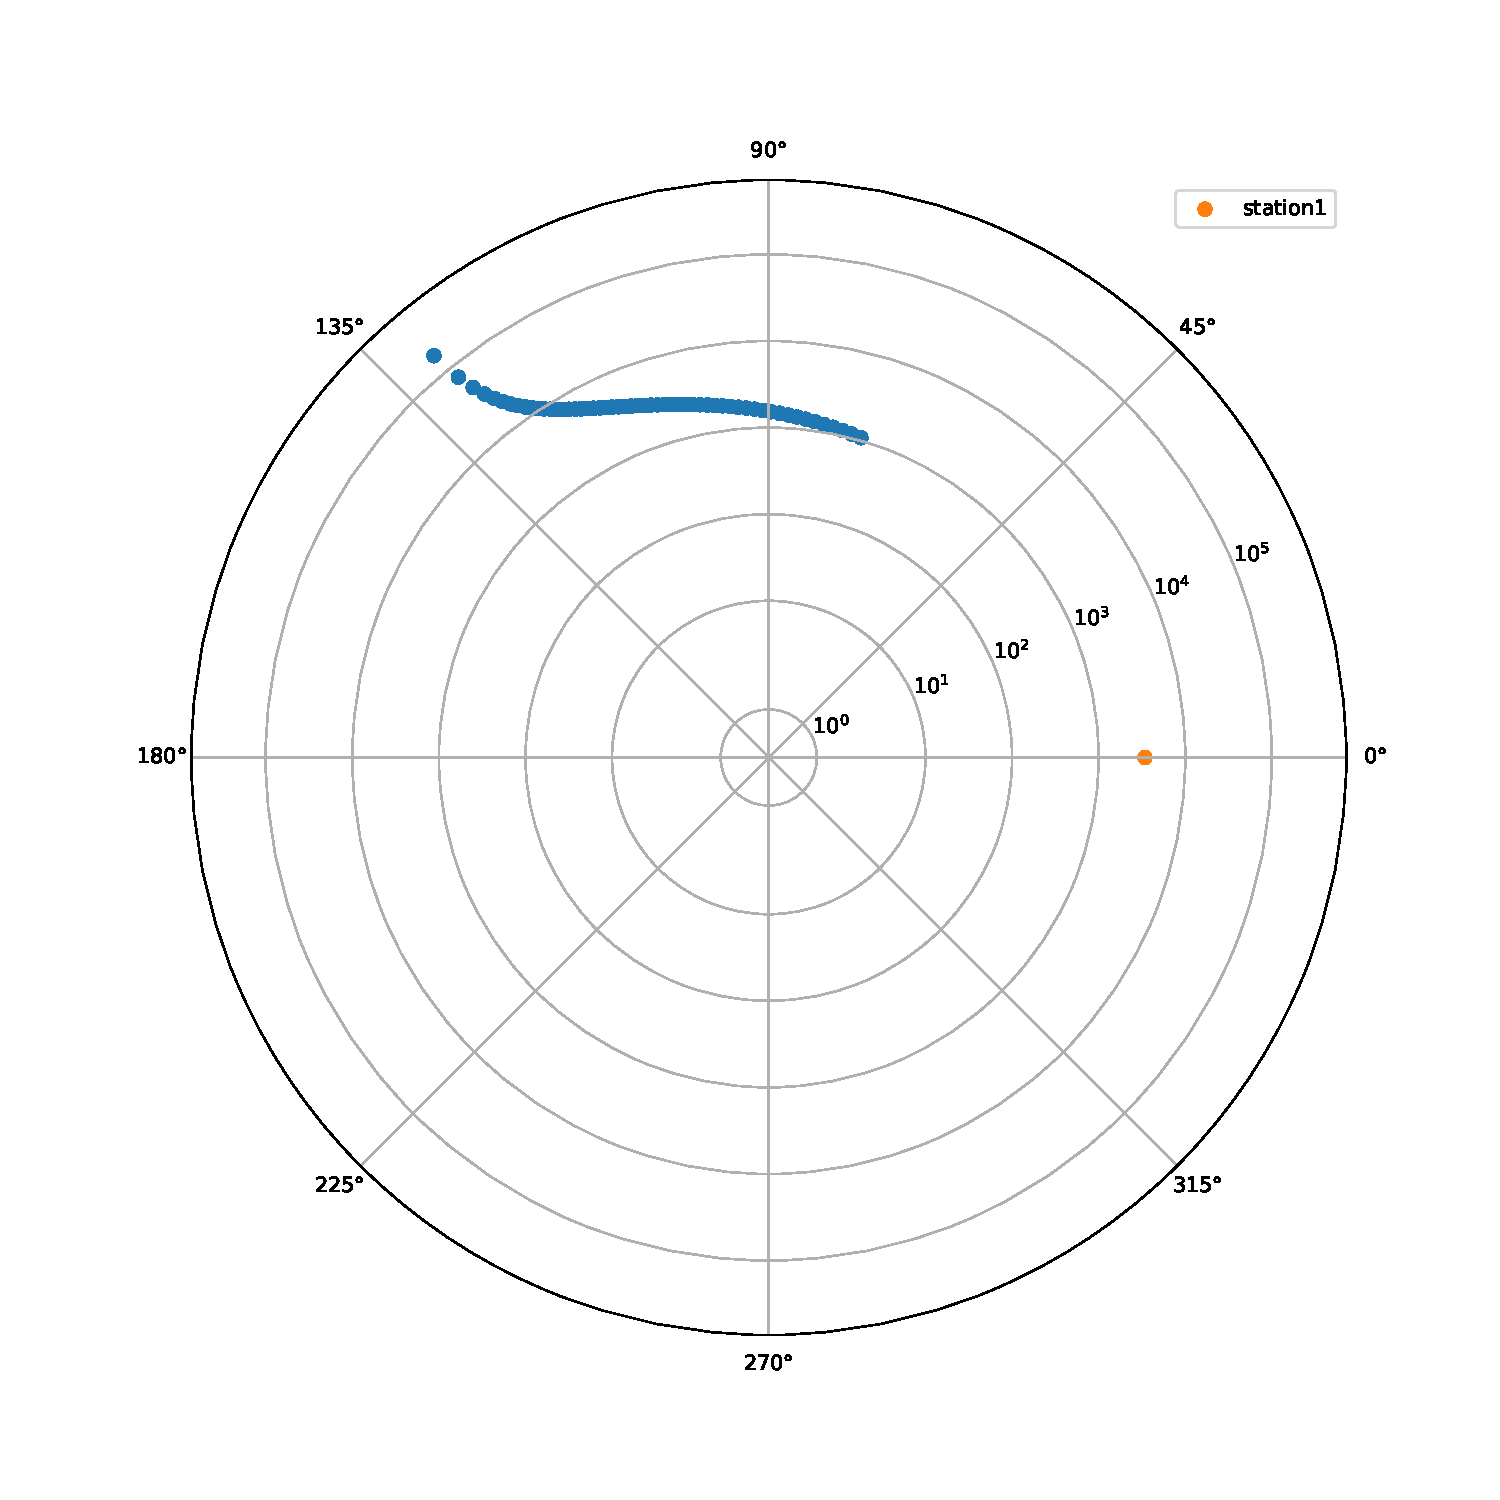
\includegraphics[width=0.4\linewidth]{data/example_plot_vertical_constrained}
	\caption{Possible incident angles and radii constrained to a maximum possible angle $\delta_{max}$}
	\label{fig:reconstruction_example_constrained}
\end{figure}
Figure \ref{fig:reconstruction_example_constrained} shows the same plot as figure \ref{fig:reconstruction_example} but with a constrained angle $\delta_{max} = \frac{\pi}{4}$.

Due to the inherent rotational symmetry of the system around the connecting straight line between both detectors, the curve shown in figures \ref{fig:reconstruction_example} and \ref{fig:reconstruction_example_constrained} show the outline of a rotational body with rotational axis equal to the connecting line. This permits a projection of the curve onto the ground in either direction. Doing this, the curves for all pairs involving a reference detector station can be calculted and projected onto the same plot, aligned according to the real world positions. Figure \ref{fig:reconstruction_example_ground} shows this construction for a coincidence $n=3$, where the reference detector is located in the center and both other detectors are located towards the right. The real world distance between the reference station and station1 is $3.4\,\text{km}$, between the reference and station2 $2\,\text{km}$.
It can be seen that the curves overlap in the bottom half of the plot, indicating a possible origin region for the primary interaction.

\begin{figure}[ht!]
	\centering
	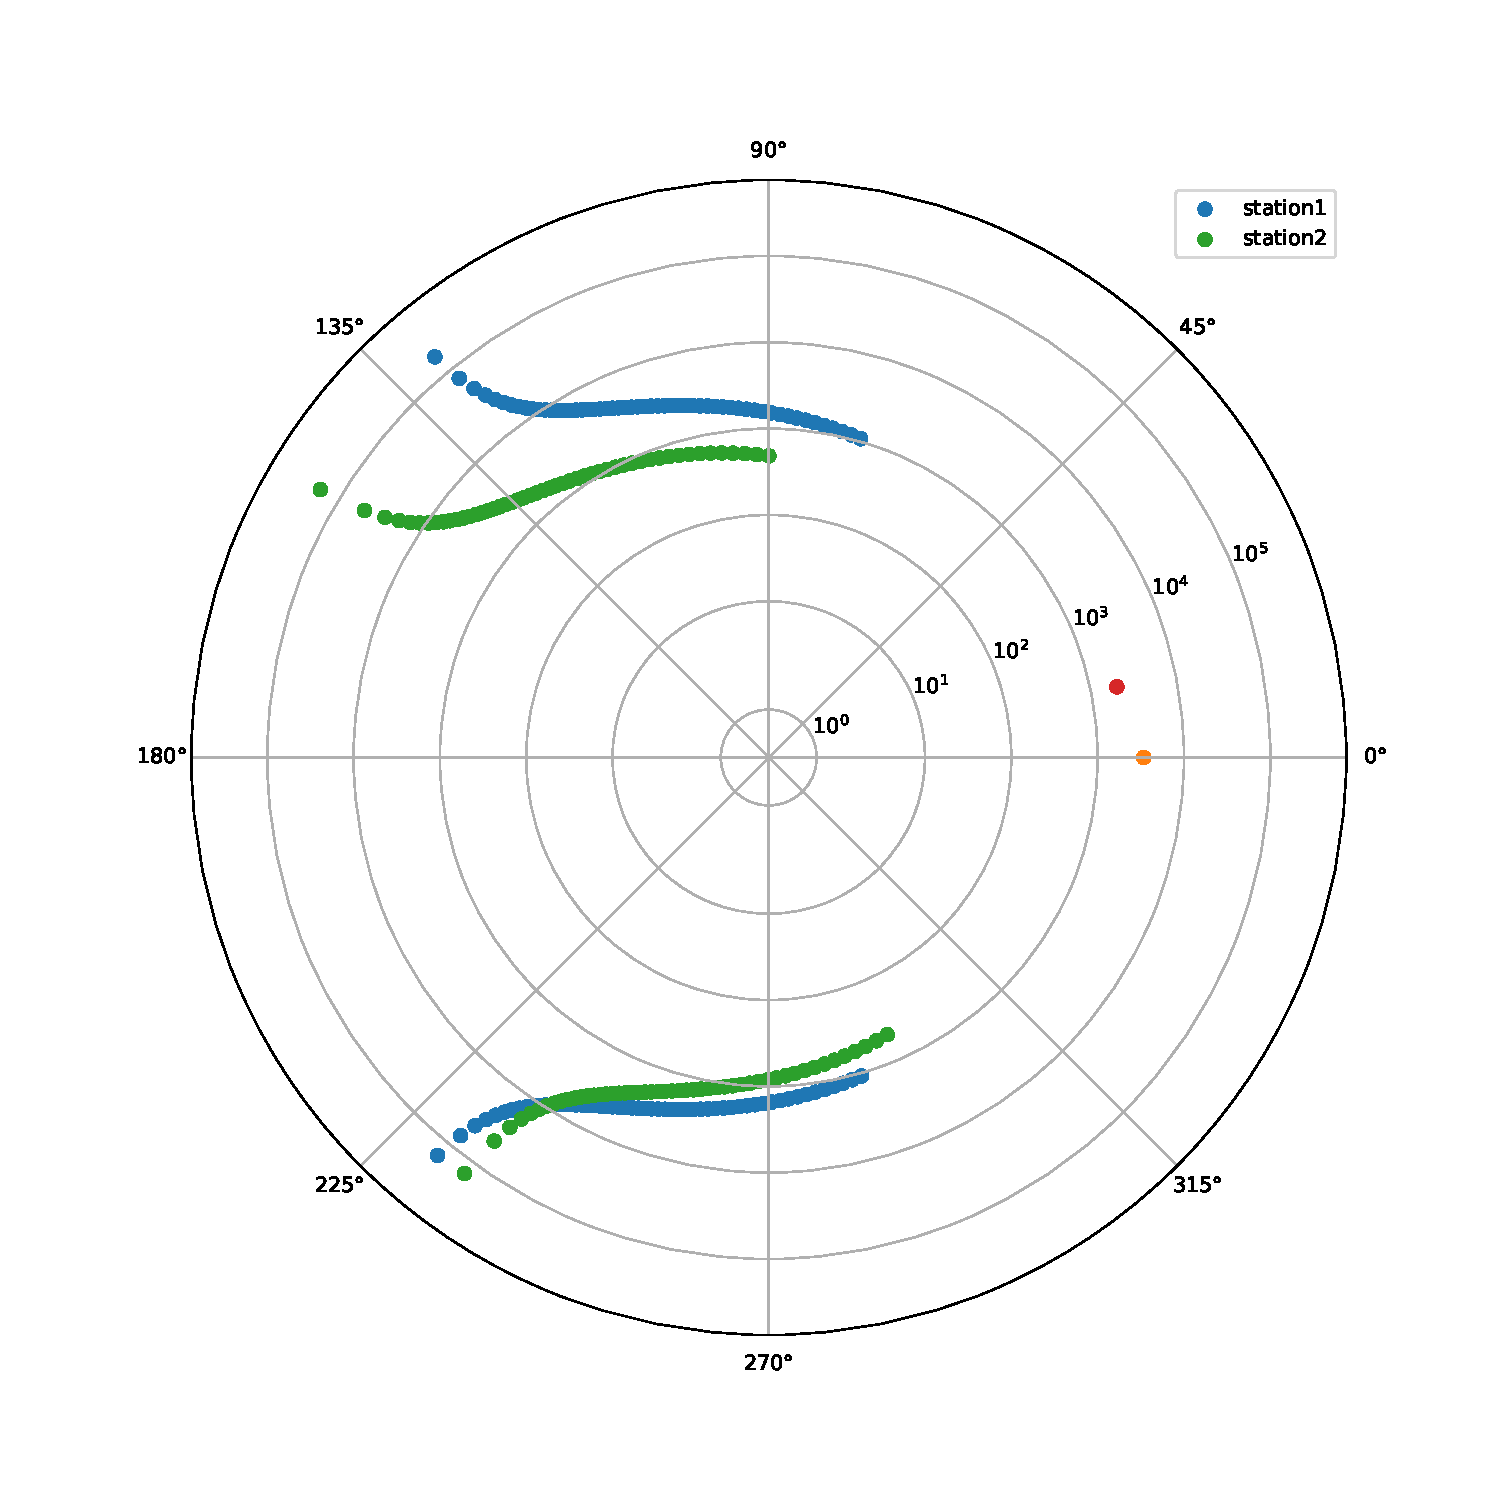
\includegraphics[width=0.4\linewidth]{data/example_plot_ground}
	\caption{Ground plot for a coincidence with $n=3$.}
	\label{fig:reconstruction_example_ground}
\end{figure}

Though due to the fact that the space of possible origin points is a rotational body, the cross section between both curves is a region in 3D space.a
\section{Program layout}
The analysis program uses a data driven pipeline design for efficient execution. It supervises itself and stores runtime data like CPU and memory usage in the database in order to be able to later review resource usage. This is useful in extrapolating the runtime impact for larger number of detector stations in the future.
An overview of the program layout for the real-time analysis is shown in Figure \ref{fig:programlayout}, the parts marked with section numbers are described in detail in their respective sections. \todo{better description of program structure}
\begin{figure}[ht!]
	\centering
	\begin{tikzpicture}[->]
		\node (source) [draw, terminal,minimum height=1cm] {Event source};
		\node (logsource) [left=of source, draw, terminal,minimum height=1cm] {Station log source};
		\node (supervision) [below=of source, draw, process,minimum height=1cm] {Station supervision (\ref{subsec:station-s})};
		\node (supervision2) [below=of supervision, draw, process,minimum height=1cm] {Time-base supervision (\ref{subsec:timebase-s})};
		\node (filter) [below=of supervision2, draw, process,minimum height=1cm] {Coincidence filter (\ref{subsec:coincidence-f})};
		\node (analysis) [right=of filter, draw, process,minimum height=1cm] {Coincidence analysis (\ref{subsec:coincidence-s})};
		\node (sink) [below=of filter, draw, terminal,minimum height=1cm] {Event Sink};

		\node (criterium) [left=of filter, draw, predproc,minimum height=1cm] {Coincidence criterium};
		
		\draw (logsource) |- (supervision);
		\draw (source) -- (supervision);
		\draw (supervision) -- (supervision2);
		\draw (supervision2) -- (filter);
		\draw (filter) -- (sink);
		\draw (filter) -- (analysis);
		\draw (supervision) -| (analysis);
		
		\draw[<->] (criterium) -- (filter);
	\end{tikzpicture}
	\caption{Program layout}
	\label{fig:programlayout}
\end{figure}
\clearpage
\subsection{Station supervision}\label{subsec:station-s}
The station supervision tracks all currently active detector stations and classifies them according to reliable and unreliable data states.
Additionally it augments each event with the location and user data which is not provided with the default event messages.

\begin{figure}[ht!]
	\centering
	\begin{tikzpicture}[->]
		\node (start) at (0,0) {};
		\node (terminal1) [below=of start,draw, terminal] {event input};
		\node (predproc1) [below=of terminal1, draw, predproc, align=left] {calculate event rate};
		\node (decide1) [below=of predproc1, draw, decision] {$\sigma\geq{k}\cdot\mu$};
		\node (terminal2) [right=of start, draw, terminal] {station log input};
		\node (decide2) [below right=of terminal2, draw, decision] {$\bar{f}_{loc}\geq1$};
		\node (decide3) [right=of predproc1, draw, decision] {$\bar{f}_{time}\geq1$};
		\node (predproc2) [below=of decide1, draw, terminal, align=left] {Mark station unreliable};
		
		
		\draw (terminal1) -- (predproc1);
		\draw (predproc1) -- (decide1);
		\draw (decide1) -- (predproc2);
		\draw (terminal2) -| (decide2);
		\draw (terminal1) -| (decide3);
		\draw (decide2) |- (predproc2);
		\draw (decide3) |- (predproc2);
	\end{tikzpicture}
	\caption{Criteria for detector station reliability}
	\label{fig:station_reliability}
\end{figure}
Figure \ref{fig:station_reliability} shows the decision process how each station is determined to be reliable. Each event is analysed and the mean event rate as well as the standard deviation of the rate is calculated continuously. If $\sigma\geq{k}\cdot\mu$ is true, where $\sigma$ is the standard deviation of the rate, $\mu$ the mean rate and $k$ a constant, the detector station is determined to have a highly unstable rate and is excluded from contributing events to the analysis.

Additionally two more factors can determine the reliability of a station. Those factors are a normed so that a value of higher than 1 causes an unreliability mark.
$\bar{f}_{time}$ is the mean time accuracy and $\bar{f}_{loc}$ the mean location precision of the \acrshort{gnss} receiver.

The time accuracy is determined through the detector station itself and results from different factors such as the \acrshort{gnss} signal quality.
The location precision is calculated through
\begin{equation*}
loc = dop\cdot\sqrt{h_{acc}^2 + v_{acc}^2}
\end{equation*}
where $dop$ is the delusion of precision, $h_{acc}$ the horizontal and $v_{acc}$ the vertical accuracy of the \acrshort{gnss} receiver. All those values are also determined in each detector station for itself. \todo{source for formula}

For all determining factors, a hysteresis is used in order to provide a more stable status of each detector station.
\begin{figure}[ht!]
	\centering
	\begin{tikzpicture}[->]
		\node (terminal1) at (0,0) [draw, terminal] {event input};
		\node (decide1) [below=of terminal1, draw, decision] {detector known};
		\node (decide2) [below=of decide1, draw, decision] {detector reliable};
		\node (decide3) [below=of decide2, draw, decision] {$f_{time}\gg1$};
		\node (predproc1) [below=of decide3, draw, predproc, align=left] {Add location info};
		\node (terminal2) [below=of predproc1, draw, terminal] {pass to coincidence filter};
		
		\node (decide1r) [right=of decide1] {no};
		\node (decide2r) [right=of decide2] {no};
		\node (decide3r) [right=of decide3] {yes};
		
		\node (terminal3) [right=of decide2r, draw, terminal] {discard event};
		
		
		
		\draw (terminal1) -- (decide1);
		\draw (decide1) -- (decide2);
		\draw (decide2) -- (decide3);
		\draw (decide3) -- (predproc1);
		\draw (predproc1) -- (terminal2);
		\draw (decide1) -- (decide1r) -| (terminal3);
		\draw (decide2) -- (decide2r) -- (terminal3);
		\draw (decide3) -- (decide3r) -| (terminal3);
	\end{tikzpicture}
	\caption{Path of an event through the station supervisor}
	\label{fig:event_station_supervisor}
\end{figure}
In figure \ref{fig:event_station_supervisor} the path of an event through the station supervisor is shown. There, only events which can be attributed to a reliable detector are accepted. Additionally, events where the time accuracy reaches extreme values are automatically discarded, since the method shown before in figure \ref{fig:station_reliability} has some inertia. This can cause single events with extremely inaccurate timestamps to artificially increase the time-base to extreme values.
\subsection{Time-base supervision}\label{subsec:timebase-s}
Since the detector network is so widely distributed, network lag and outages can introduce considerate deviations in arrival times between event messages from different detector stations. Consider the scenario shown in figure \ref{fig:network-topology}. There detector stations $A$, $B$ and $C$ all have different network delays to the server and so the event timestamps marked with $t_{A,B,C}$ have different arrival times at the server marked as $t'_{A,B,C}$. That necessitates a considerably larger sample interval for the coincidence determination than the expected coincidence interval.
\begin{figure}[ht!]
	\centering
	\begin{tikzpicture}
		\node (server) [networknode] at (6.5,5) {Server};
		\node (serverbl) [below left=of server] {};
		\node (serverbr) [below right=of server] {};
		\node (servera) [above=of server] {};
		\node (a) [networknode, above=of servera] {A};
		\node (b) [networknode, below right=of serverbr] {B};
		\node (c) [networknode, below left=of serverbl] {C};
		
		\path[draw]
			(a) edge node[left] {$100\,\text{ms}$} (server)
			(b) edge node[above right] {$10\,\text{ms}$} (server)
			(c) edge node[left] {$35\,\text{ms}$} (server)
			;
			
			\draw[decoration={%
				discontinuity,
				amplitude=5,
				meta-segment length=2,
				segment length=3},
			decorate, ultra thick] (0,0) -- (10,0);
			\draw[ultra thick, ->] (10,0) -- (13,0) node[below] {$t$};
			\draw[dashed] (1,0.5) -- ++(0,-1) node[below] {$t_A$};
			\draw[dashed] (3,0.5) -- ++(0,-1) node[below] {$t_B$};
			\draw[dashed] (4,0.5) -- ++(0,-1) node[below] {$t_C$};
			
			\draw[dashed] (6,0.5) -- ++(0,-1) node[below] {$t_B'$};
			\draw[dashed] (7,0.5) -- ++(0,-1) node[below] {$t_C'$};
			\draw[dashed] (10,0.5) -- ++(0,-1) node[below] {$t_A'$};
	\end{tikzpicture}
	\caption{Network topology of detector network}
	\label{fig:network-topology}
\end{figure}

The time-base supervisor determines a baseline waiting interval by observing the maximum time difference between event timestamps over a certain sample time interval. A value of $2\,\text{s}$ proved experimentally to provide a good balance between runtime impact, stability and reaction time. In the case of a total network outage for one detector station however, the events will be buffered locally in the station and transmitted at a later time when the network connection has been re-established. This can mean delays of up to a few minutes and would lie outside the two second time-base and a loss of data would be the result. In order to mitigate this, an attempt to predict network outages is implemented by observing the current event rate in relation to the mean event rate over a long sample time. A factor is calculated through
\begin{equation*}
	f = max(1, \frac{\mu_{r} - r}{\sigma_{r}})
\end{equation*}
where $r$ is the current event rate, $\mu_{r}$ the mean rate and $\sigma_{r}$ the standard deviation of the rate over a long sample time. This factor is then relative to the expected event rate of the detector station and is always greater or equal to 1. This is calculated for all detector stations and the maximum value is used as a scaling factor for the previously described time-base.

The resulting time value can then be used by the coincidence filter as a timeout value for the construction of coincidence events.
\subsection{Coincidence filter}\label{subsec:coincidence-f}
The coincidence filter inspects each event in order to find all possible coincidences. It does so by creating so-called event constructors which hold the event and information about the creation time and the specific per-constructor timeout period. The timeout is taken from the timebase supervisor described in section \ref{subsec:timebase-s}. It is updated each time a more recent and higher value is received. When the timeout is passed, the constructor is committed in order to send the constructed event off for further processing. The flow of an event through the coincidence filter is shown in figure \ref{fig:coincidence-flow}.
\begin{figure}[ht!]
	\centering
	\begin{tikzpicture}[->]
		\node (terminal1) at (0,0) [draw, terminal] {START};
		\node (decide1) [below=of terminal1, draw, decision] {constructor available};
		\node (predproc1) [below=of decide1, draw, process, align=left] {select next constructor};
		\node (decide2) [below=of predproc1, draw, decision] {criterium met};
		\node (predproc3) [right=of decide2, draw, predproc] {create new constructor};
		\node (predproc2) [below=of decide2, draw, predproc] {add event to constructor};
		\node (terminal2) [below=of predproc2, draw, terminal] {END};
		
		\node (decide1r) [right=of decide1] {no};
		\node (decide2l) [left=of decide2] {no};
		
		
		\draw (terminal1) -- (decide1);
		\draw (decide1) -- (predproc1);
		\draw (predproc1) -- (decide2);
		\draw (decide2) -- (predproc2);
		\draw (predproc2) -- (terminal2);
		\draw (decide2) -- (decide2l) |- (decide1);
		\draw (decide1) -- (decide1r) -| (predproc3);
		\draw (predproc3) |- (terminal2);
	\end{tikzpicture}
	\caption{Flow of an event through the coincidence filter}
	\label{fig:coincidence-flow}
\end{figure}
\begin{figure}[ht!]
	\centering
	\begin{tikzpicture}[->]
		\node (terminal1) at (0,0) [draw, terminal] {START};
		\node (decide1) [below=of terminal1, draw, decision] {constructor available};
		\node (process1) [below=of decide1, draw, process, align=left] {select next constructor};
		\node (process2) [below=of process1, draw, process, align=left] {update timeout value};
		\node (decide2) [below=of process2, draw, decision] {timed out};
		\node (process3) [below=of decide2, draw, process] {commit coincidence};
		
		\node (decide1r) [right=of decide1] {no};
		\node (decide2l) [left=of decide2] {no};
		
		\node (terminal2) [right=of decide1r, draw, terminal] {END};
		
		
		\draw (terminal1) -- (decide1);
		\draw (decide1) -- (process1);
		\draw (process1) -- (process2);
		\draw (process2) -- (decide2);
		\draw (decide2) -- (process3);
		\draw (process3) -- ++(-4,0) |- (decide1);
		\draw (decide1) -- (decide1r) -- (terminal2);
		\draw (decide2) -- (decide2l) |- (decide1);
	\end{tikzpicture}
	\caption{Timeout update and committing of event constructors}
	 \label{fig:event-constructors}
\end{figure}
\subsection{Coincidence analysis}\label{subsec:coincidence-s}
The coincidence analysis creates a graph with data for all detector station combinations. It records a histogram of the coincidences between each station pair as well as joined uptime and total number of coincidences.
The histograms use a bin size which is calculated per detector pair depending on their distance so that the interesting data is properly resolved with a total number of 2000 bins.
\clearpage
\section{Conclusion}
\clearpage

\makeback
\end{document}
